\documentclass[iop]{emulateapj}

\usepackage{amsmath,amssymb}
\usepackage{color}
\usepackage{natbib}
\usepackage{graphicx}
\usepackage{hyperref}
\usepackage{ulem}
\usepackage{adjustbox}
\usepackage[draft]{todonotes}

\newcommand\toplotrm[1]{\todo[color=green, inline, size=\small]{Plot: #1}}
\newcommand\towriterm[1]{\todo[color=yellow, inline, size=\small]{Write: #1}}
\newcommand\todorm[1]{\todo[color=cyan, inline, size=\small]{To do: #1}}

\newcommand\toplotemh[1]{\todo[color=pink, inline, size=\small]{Plot: #1}}
\newcommand\towriteemh[1]{\todo[color=orange, inline, size=\small]{Write: #1}}
\newcommand\todoemh[1]{\todo[color=red, inline, size=\small]{To do: #1}}

\newcommand\towrite[1]{\todo[color=gray, inline, size=\small]{Write: #1}}
\newcommand\rmcomment[1]{\textcolor{red}{(RM: #1)}}
\newcommand\emhcomment[1]{\textcolor{blue}{(EMH: #1)}}

\citestyle{aa}

\shorttitle{Meta-Calibration} \shortauthors{Huff and Mandelbaum}

\begin{document}
\title{Meta-Calibration: Direct Self-Calibration of Biases in Shear Measurement}
\author{Eric M. Huff\altaffilmark{1}}
\author{Rachel Mandelbaum\altaffilmark{2}}

\altaffiltext{1}{Jet Propulsion Laboratory, 
4800 Oak Grove Drive, Pasadena, CA 91109, USA}
\altaffiltext{2}{McWilliams Center for Cosmology, Department of Physics, Carnegie Mellon University,
  Pittsburgh, PA 15213, USA}

\keywords{cosmology: observations --- gravitational lensing: weak ---
  methods: observational}

\begin{abstract}
  One of the primary limiting sources of systematic uncertainty in forthcoming weak lensing
  measurements is systematic uncertainty in the quantitative relationship between the distortions
  due to gravitational lensing and the measurable properties of galaxy images. We present a
  statistically principled, general solution to this problem. Our technique infers multiplicative
  shear calibration parameters by modifying the actual survey data to simulate the effects of a known
  shear. It can be applied to any shear estimation method based on weighted averages of galaxy shape
  measurements, which includes all methods used to date for shear estimation with real data.  Use of
  the real images mitigates uncertainty due to unknown galaxy morphology, which is a serious concern
  for calibration of shear estimates based on image simulations.  We test our results on simulated
  images from the GREAT3 challenge, and show that the method eliminates calibration biases for
  several different shape measurement techniques at the level of precision measurable with the
  GREAT3 simulations (a few tenths of a percent).
\end{abstract}

\section{Introduction}

Accurate measurement of weak gravitational lensing offers the most
direct probe of the dark sector of the universe
\citep[e.g.,][]{2001PhR...340..291B,2003ARA&A..41..645R,schneider06,2008ARNPS..58...99H,2010RPPh...73h6901M,2013PhR...530...87W}.
Weak lensing measurements are thus a core part of the international
cosmology program, and a key science driver for several wide-field
astronomical imaging cameras and associated surveys -- the Kilo Degree
Survey\footnote{\url{http://kids.strw.leidenuniv.nl}}
\citep{KiDS_main}, the Dark Energy Survey \citep{DES_main}, the
Hyper Suprime-Cam and associated survey\footnote{\url{http://hsc.mtk.nao.ac.jp/ssp/}}
\citep{HSC_main}, LSST\footnote{\url{http://www.lsst.org/lsst/}}
\citep{2009arXiv0912.0201L},
Euclid\footnote{\url{http://sci.esa.int/euclid/}\url{http://www.euclid-ec.org}}
\citep{2011arXiv1110.3193L}, and
WFIRST\footnote{\url{http://wfirst.gsfc.nasa.gov}}
\citep{2015arXiv150303757S}.

Despite this investment, the weak lensing community has more work to
do in order to ensure that the algorithms for inferring shear are
unbiased at the required levels to avoid systematic errors from
dominating over the statistical errors. One of the largest such
systematic error sources is the {\it shear calibration bias}, the
quantitative relationship between the true gravitational lensing shear 
and its observables as estimated from the ensemble of galaxies in the survey.

In the weak shear limit that is most relevant for wide-field cosmology, the
gravitational lensing signal can be described as a linear
transformation
$\boldsymbol{A}\mathbf{x}_{\rm true} = \mathbf{x}_{\rm obs}$ between
the lensed and unlensed image coordinates, parameterized by two shears
$(\gamma_1,\gamma_2)$ and a convergence $\kappa$
\begin{align}
\begin{pmatrix}
1 + \kappa + \gamma_1 & \gamma_2 \\
\gamma_2 & 1 + \kappa - \gamma_1
\end{pmatrix}
\end{align}.
The major observable effect of weak lensing is to perturb the measured
ellipticities $\mathbf{e} = (e_1,e_2)$ of galaxies. At large
separations, these shapes no know preferred direction, so the mean
$\mathbf{e}$ should vanish over a wide enough field. Weak lensing
studies exploit this intrinsic symmetry, and search for spatially
coherent anisotropies in the ensemble of observed galaxy shapes
arising from lensing distortions produced by foreground matter.

The effects of the shear and convergence on this observable cannot be
straightforwardly distinguished, so the fundamental quantity
constrained by lensing is the reduced shear
\begin{align}
 g = \frac{\gamma}{1 - \kappa}.
\end{align}

The responses of individual galaxy images to $g$ vary depending on
the choice of ellipticity measure and the intrinsic shape and
orientation of each galaxy. Lensing studies rely on ensemble averages
of galaxy ellipticities, and the shears are weak enough that these ensemble averages usually respond
linearly to an applied (reduced) shear, so it is conventional to define the shear
calibration parameters as
\begin{align}
\mathbf{e} = (1 + m) \mathbf{g} + \mathbf{c}
\label{eqn:calibPars}
\end{align}
where $\mathbf{e}$ and $\mathbf{g}$ are ensemble-averaged shears and
ellipticity measures, respectively. \rmcomment{Might be better to explicitly use the $\langle\rangle$
  since this is conventional notation?} Generally, $\mathbf{c}$ is a
result of measurement biases (such as an incomplete correction for the
point-spread function) that introduce a preferred direction in the
image plane. It can in principle  be known or removed with sufficient
knowledge of the experiment. $m$ depends in part on the ensemble of
(unobserved) galaxy properties, so it is impossible in principle to
know exactly {\it a priori} (though \citealt{2014MNRAS.438.1880B} show
how to derive this information for their proposed shear estimator from
deeper calibration fields). \rmcomment{That only works because they don't use an ensemble average over
  ellipticities, though.  So I think this aside is somewhat tangential to the main point, or at
  least deserves further qualification.}


In practice, a nonlinear response generically introduced by the algorithms
used for measurement of $\boldsymbol{e}$ can introduce both
multiplicative and additive biases in a manner that interacts with the
unknown true ensemble properties of galaxies
\citep{2007MNRAS.380..229M,2011MNRAS.414.1047Z}, and are very
difficult to predict from first principles. For this reason, the weak
lensing community has organized a series of blind measurement
challenges, where participants attempted to extract an unkown lensing
signal from simulated images.  The earliest of these were the first
two Shear TEsting Programmes \citep[STEP1,
STEP2]{2006MNRAS.368.1323H,2007MNRAS.376...13M}. The results made two
things clear: that lensing measurement algorithms needed to improve in order to avoid being
systematics-dominated,
and that shear measurement was sufficiently complex that successive
simulation challenges should focus on a subset of the issues.

The next round of simulation challenges -- GREAT08, GREAT10, and GREAT3
\citep{2009AnApS...3....6B,2013ApJS..205...12K, 2015MNRAS.450.2963M} --
embraced a narrower focus and saw significant performance
improvements. They also drove improvements in our understanding of 
various sources of bias in shear estimation, which is of use in future
algorithmic development.  The best-performing algorithms from the most
recent challenge, GREAT3, reduced $m$ and $c$ to levels approaching
those needed for the most ambitious planned lensing measurements,
albeit with simulations that did not include all the features of real
data.


While this was certainly good news, the narrowed focus of the GREAT
challenges necessarily left some of the most important sources of
lensing calibration bias untouched. Remaining issues of significant
concern include biases resulting from:
\begin{itemize}
\item object detection and selection
\item deblending
\item wavelength-dependent effects
\item instrumental defects and nonlinearities
\item star-galaxy separation
\item non-white pixel noise
\item cosmic rays and other image artifacts
\item redshift-dependent calibration biases
\item shear estimation for low-resolution and/or low signal-to-noise ratio ($<12$) galaxies
\end{itemize}
The impact of these factors depends strongly on the specifics of the
experiment. For this reason, shear calibration in current and future
experiments relies heavily on simulations designed to match the
properties of each experiment
\citep{KiDS450,2016MNRAS.tmp..827J}. Such external simulations are
always limited in their realism:  accurately modeling everything
relevant about the experiment turns out to be extremely difficult. Showing that a given simulation suite
is adequate for calibrating a lensing measurement is a formidable
challenge in its own right (c.f.\ the Ultra Fast Image Generation
simulations described in \citealt{2013A&C.....1...23B}, or the
calibration simulations used for the KiDS weak lensing cosmology in
\citealt{2016arXiv160605337F}).

The method outlined in this paper is motivated by the observation
that introducing a synthetic shear signal into real data is much
easier than building a realistic comprehensive first-principles simulation
suite. Perturbing the actual data automatically incorporates features
present in real images (e.g., image artifacts, selection biases,
unusual high-redshift galaxy morphologies) that are otherwise
difficult to accurately simulate.  It enables the determination of how the {\em real galaxy
  population} in the data responds to a shear directly and empirically.

% \rmcomment{I think that it depends what kinds of features you are talking
 % about.  For example, cosmic rays that impinge on the objects will get deconvolved and reconvolved
 % with shear and a larger PSF, so their impact won't be quite right.  We should at some point
 % acknowledge that their inclusion isn't 100\% perfect (but it is still likely better than trying to
 % simulate all of these from first principles).}

We have implemented this concept, which we call metacalibration, using
the public GalSim \citep{2015A&C....10..121R} image simulation
package, and designed our algorithm to wrap an arbitrary external
shear estimation module, provided that it functions by estimation of per-galaxy ellipticities and
then estimates the ensemble shear through weighted averages. We test our technique on simulated GREAT3
image data, and find that it successfully calibrates several older shear
estimation methods to a level of accuracy comparable to the
best-performing algorithms from the GREAT3 challenge. We also
demonstrate that our algorithm can detrend additive biases resulting
from incomplete point-spread function (PSF) corrections by introducing synthetic PSF
ellipticity.  We make our metacalibration scripts available for
general use.

\section{Method}
There are three layers to the shear calibration method we propose
here. The first is the generation of the modified images using a procedure similar to one proposed
in \cite{2000ApJ...537..555K}.
% Note from RM: removed use of phrase "counterfactual images" before it was defined below.
 We use the GalSim package
\citep{2015A&C....10..121R} to modify real astronomical images by
adding synthetic shear and PSF distortions of known amplitude. These
modified images are counterfactuals; they are a model for what would
have been observed under (nearly) the same image quality conditions,
on the same galaxies, with a different shear. If the measurement
process is repeated on the counterfactual images, the result gives an
accurate estimate of shear calibration biases.

The second layer is the choice of ellipticity measure used to estimate per-object shapes. This step is
the primary focus of most studies that address shear
calibration biases. Here we are agnostic about the choice of
measurement algorithm; as long as the algorithm is sufficiently
well-behaved (in a manner that we will describe in Sec.~\ref{subsec:shapemeas}), the image
manipulation step can be used to generate an accurate shear
responsivity.

The final layer is the choice of averaging mechanism to estimate the response of the ensemble shear
estimate to an applied shear. Noise properties
of shape measurements can vary widely depending on the shape measurement method, which entails similar variation in
the metacalibration estimates for shear responsivity. For the cases we
describe below, an optimal strategy for ensemble averaging produces
significant gains over more straightforward averaging schemes.

\subsection{Generating a Counterfactual Image}
\label{sec:counterfactual}
Fortunately, for the weak shears under consideration in most
cosmological survey applications, the relationship between the shear
and the galaxy shapes (or related observables) is very close to
linear, so accurate shear calibration requires only the first
derivative of the galaxy properties with respect to the shear. What
follows is a method for estimating this derivative directly from the
images. Throughout we will assume that the observed image
$I({\mathbf{x}})$ is equal to the unsmeared galaxy image
$G(\mathbf{x})$ convolved with some point-spread function (including the
atmospheric seeing, the optical PSF, and the pixel response function) $P(\mathbf{x})$.

In an ideal world, we would vary the gravitational shear experienced
by the image before is smeared by $P$, constructing the counterfactual
image $I'(\mathbf{x}| {\boldsymbol g})$:
\begin{equation}
  I'({\mathbf{x}}|\mathbf{g}) = P \ast\left( \hat{\mathbf{s}}_{\mathbf{g}}G\right)
\end{equation}
where $\hat{\mathbf{s}}_{\boldsymbol g}$ is the shear operator that
produces the reduced shear $\mathbf{g}$, as in
e.g.~\cite{2002AJ....123..583B}. The shear sensitivity of the image
would then be a straightforward numerical derivative of $I'$ with
respect to $\mathbf{g}$, and the shear sensitivity of an ellipticity
measure $\mathbf{e}$ can be got from measurements on multiple . \rmcomment{this sentence trails off
  without ending; what was this supposed to say?} We can
even write down a procedure for producing $I'$ from $I$ if we know
$P$:
\begin{equation}
  I'({\mathbf{x}}) = P \ast \left[\hat{\mathbf{s}}_\mathbf{g}\left( P^{-1} \ast I \right)\right].
\end{equation}
The noise in $I$ has finite power on scales where $P$ is small or
vanishing. Deconvolution amplifies noise, and because of the shear,
this is not cancelled for all Fourier modes by reconvolution with $P$.  The noise
amplification can be mitigated by reconvolving after the shear
operation with a new PSF $\Gamma$ (instead of $P$), constructing
$\Gamma$ so that it suppresses the noise amplification that is
produced by the deconvolution operation.

All that is required for $\Gamma$ is that (in Fourier space, with the
tilde indicating the Fourier transformed quantity)
$\|\tilde{\Gamma}(\mathbf{|k|}) \| \geq
\|\hat{\mathbf{s}}\tilde{P}(\mathbf{k})\|$
for all $\mathbf{k}$.  This condition can be achieved  without introducing additional
PSF anisotropy by choosing
$\Gamma(\mathbf{x}) = P\left((1+2|\gamma|)\mathbf{x}\right)$.

Our chosen procedure for producing a sheared counterfactual image is
\begin{equation}
I' = \Gamma \otimes \left[\hat{\mathbf{s}}_\mathbf{g} \left(P^{-1} I \right)\right].
\end{equation}
This procedure clearly requires a good model for $P$, but so do all
shear measurements. PSF model errors enter at the
same order in measurements on the resulting image that they would in
an unmodified image.

Once the counterfactual image $I'(\mathbf{x}|\mathbf{g})$ with
$\|\mathbf{g}\| \ll 1$ has been created, the galaxy detection and
shear measurement pipeline should be rerun. This provides a measure of
the shear sensitivity -- not for the original image, but for an image
with the PSF $\Gamma$. This requires that the full measurement -- not
just the sensitivity analysis -- be run on an additional
counterfactual image $I'(\mathbf{x}|\mathbf{g}=0)$, so that the numerical
derivative $\frac{\partial I'}{\partial \mathbf{g}}$ is well-defined.

This procedure introduces anisotropic correlated noise, which can
produce a systematic multiplicative shear bias. If the noise
properties of the initial image are known, the noise anistropy can be
removed with the addition of further anisotropic correlated noise (with power spectrum carefully chosen). As we describe below, we
have not found noise isotropization to be a necessary step for the
images that we used for testing.  These have an effective $S/N$ limit
of $\sim 12$. The forthcoming Sheldon et al.~(2016) will investigate the
effects of the anisotropic correlated noise at lower signal-to-noise ratios, and
describe effective mitigation procedures.

Metacalibration can be used to mitigate other systematics as
well. Even those measurement methods with the highest scores in the
GREAT3 lensing challenge were unable to completely remove the effects
of PSF ellipticity on the inferred shear. We can introduce an
artifical PSF anisotropy by replace $\Gamma$ with a PSF containing the
desired synthetic distortion.  We show below that reconstructing
images with added PSF ellipticity, rather than added shear, allows us
to de-trend some of the bias due to PSF anisotropy. A similar approach
could be used to measure calibration biases arising from any effect --
signal or systematic error -- that can be simulated by perturbing the
images as above.


\subsection{Shape Measurement Algorithms}
\label{subsec:shapemeas}
Accurate ensemble shears can only be derived through measurement of the counterfactual
images described above if the shape measurement algorithm is
sufficiently well-behaved. Here, that entails the requirement that the
quantity reported by the shape measurement algorithm be linear in the
underlying shear in the regime relevant for the measurement. \rmcomment{I'm not sure that's true on
  a per-object basis, as long as it's true for the ensemble?  Same comment is relevant on the next
  paragraph.  I mean, the standard ellipticity and distortion do not have a linear shear response on
a per-object basis, only for the ensemble.}

We test a variety of shape algorithms below that make use of differing
definitions of ellipticity. As we are attempting to construct a shear
calibration procedure that is agnostic about the choice of per-object shape measurement 
algorithm, and which only requires that we use a measured galaxy
property with approximately linear sensitivity to shear (called a
shape measure), we will use $\mathbf{e}$ below to signify all of the
shape measures discussed in this paper, regardless of their precise
definition.

\subsection{Ensemble Shear Inference}
Counterfactual images can in principle be used to derive a per-object shear
response for a modified version of the original image.  
However, the quantities of interest in Eq.~\ref{eqn:calibPars}
are ensemble responses.  Hence it is necessary to run the ensemble shear inference step on the
counterfactual images, in order to get the shear responsivity of the ensemble shear estimate. 

\emhcomment{It's really not clear when averaging should work, and when
it fails why the histogram estimator should work instead. We have
precious little theory at this point about when our proposed
procedure should be expected to break. }

\section{Implementation}
\subsection{Image Modification}
We use
GalSim\footnote{\url{https://github.com/GalSim-developers/GalSim}} to
manipulate the images and to generate simulations for validation. For
each galaxy, we create nine modified images: two for each of the two
shear components, two for each of the two PSF ellipticity components,
and one for the final measurement using the enlarged PSF $\Gamma$ (two-sided derivatives with
respect to shear and PSF ellipticity were found to be less noisy than one-sided derivatives). 
We run the provided shape
measurement pipeline on each of these images, and the results are used
to construct a set of finite difference estimates of shear calibration and
additive PSF biases.

This sort of image manipulation is trivial to carry out using GalSim; 
we rely on the rigorous testing of the
image convolution, interpolation, and resampling algorithms that the
development team performed to enable the GREAT3 shear testing
simulations.  From the perspective of numerical validation, the tests
in section~9 of \cite{2015A&C....10..121R} illustrate that GalSim can
accurately render sheared images of quite complex galaxy and PSF light
profiles with its default settings that control numerical accuracy.

For each galaxy and PSF postage stamp, we first create an
\texttt{InterpolatedImage} object. This object is deconvolved by the
PSF model (including the pixel response). For the shear finite
differences, we apply a small shear $\Delta\mathbf{g}$ (typically 1\%) to
the resulting deconvolved image. The original PSF is dilated by twice
the shear distortion to produce $\Gamma$, and then re-convolved with
the sheared deconvolved image. This reconvolved, sheared image is then
passed to the shape measurement routine, along with the image
representation of the new, enlarged PSF $\Gamma$. For the PSF
sensitivity, we follow a similar procedure, but shear the dilated PSF
image rather than the deconvolved galaxy image. Finally, we create a
reconvolved image with no added shear but with the PSF $\Gamma$, on
which we perform the final shape measurement.

\rmcomment{In everything below, we are still kind of conflating the per-object responses with
  ensemble responses.  We should be very clear and specific about what things we could choose to
  construct (but don't really use) vs.\ which ones we actually do use in practice. }

Shape measurements on these images are used to derive shear
calibration and PSF biases {introduced by the chosen shape measurement
  method}. The shapes measured from the sheared reconvolved images
with positive and negative applied shears, $\mathbf{e}_{+}$ and
$\mathbf{e}_{-}$, can be used for a straightforward finite-difference
estimate of the multiplicative shear calibration
\begin{align}
R &= \frac{\partial \mathbf{e}}{\partial \mathbf{g}}  \\
 &=\frac{\mathbf{e}_{+} - \mathbf{e}_{-}}{2\Delta\mathbf{g}}
\end{align}
Additive biases introduced by the shape measurement are related to the
sum of these two quantities:
\begin{align}
\mathbf{c} &= \frac{\mathbf{e}_{+} + \mathbf{e}_{-}}{2} - \mathbf{e}
\end{align}
and if the shape measurement algorithm does not perfectly remove PSF
ellipticity, then the shapes measured from shearing the PSF
($\mathbf{e}_{+,\rm PSF}$ and $\mathbf{e}_{-,\rm PSF}$) permit calculation
of at least the linear-order residual PSF ellipticity biases:
\begin{align}
R_{\rm PSF} = \frac{\mathbf{e}_{+,\rm PSF} - \mathbf{e}_{-,\rm PSF}}{2\Delta\mathbf{g}}.
\end{align}
The result of this process is a catalog of shear responsivities, PSF
responsivities, and additive biases for every galaxy. A histogram of
these quantities is shown in figure~\ref{fig:calibhist}. The derived
biases and responsivities are very noisy, so attention must be paid to
how inference is performed on the full ensemble of galaxies. 
\rmcomment{It's not really clear to me how useful this is, considering that we don't use these
  directly, and the level of noise etc.\ must surely depend on the shape measurement method?  Unless
  you want to specifically use this to motivate the use of the histogram estimator?}

\begin{figure*}
\begin{center}
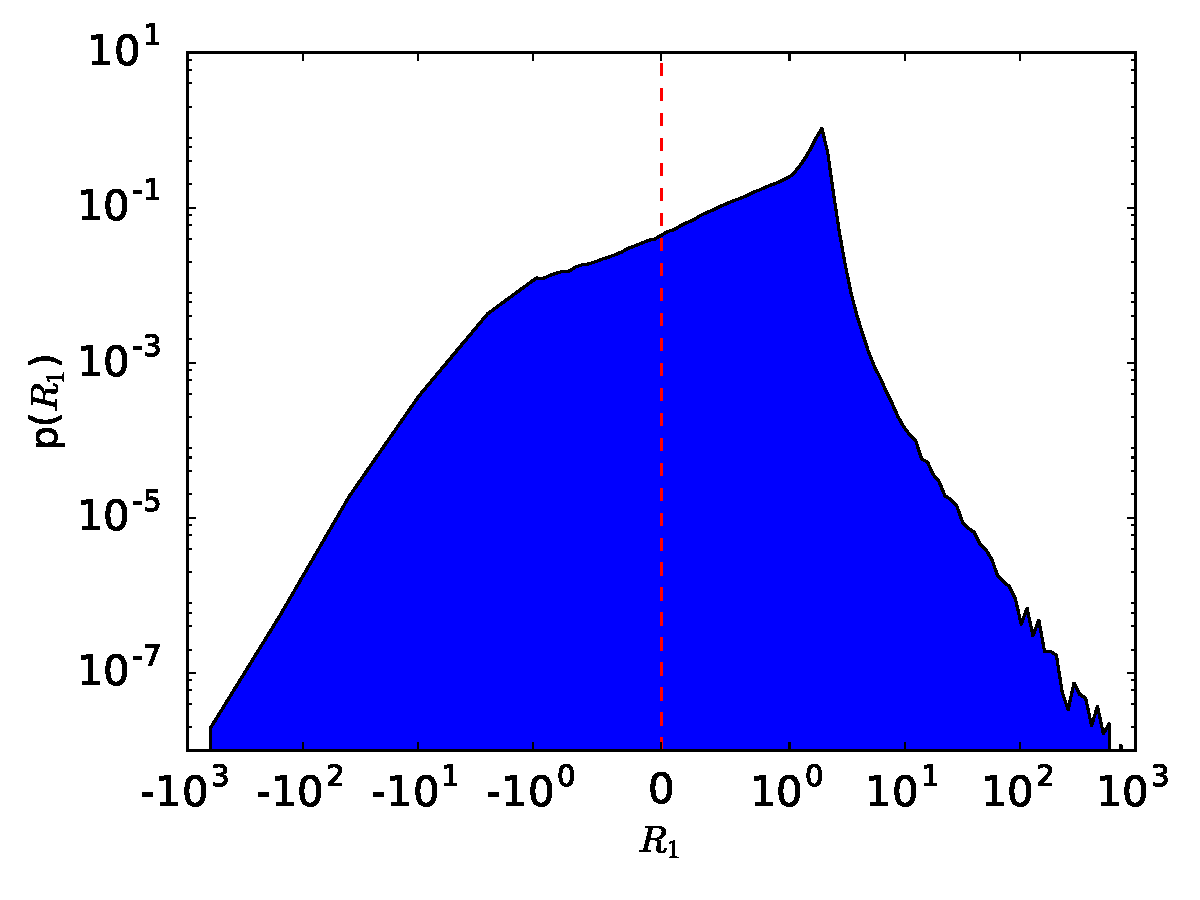
\includegraphics[width=0.45\textwidth]{./Plots/R1_hist.pdf}
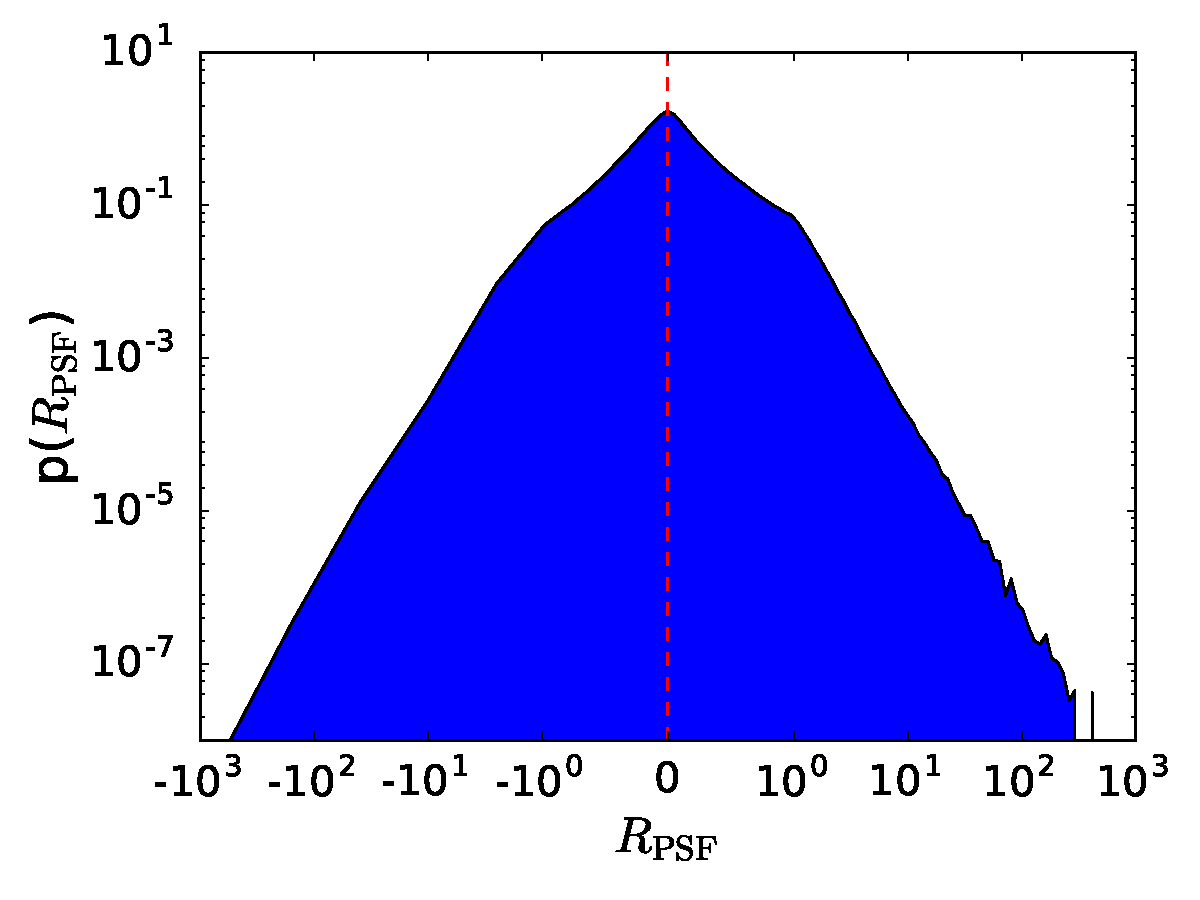
\includegraphics[width=0.45\textwidth]{./Plots/a1_hist.pdf}
\end{center}
\caption{{\bf Left:} Normalized distribution of meta-calibration shear
  responsivities from regaussianization, on the
  Control-Ground-Constant branch of the GREAT3 simulations.  {\bf
    Right:} Distribution of meta-calibration PSF ellipticity
  responsivities from regaussianization, on the
  Control-Ground-Constant branch of the GREAT3 simulations. A
  vertical red dashed line is drawn for reference at the expected
  responsivity for perfectly round objects, $R=2$, in the left
  panel. }
\label{fig:calibhist}
\end{figure*}


\subsection{Shear Estimation Algorithms}

Since the metacalibration method can in principle be used to calibrate
shears from any shear estimation algorithm derived using an average of per-object shapes, we chose three easily
available shear estimation methods, all of which are implemented in
GalSim.  Two of these methods are traditional shear estimation
methods that have somewhat different assumptions but are both based on
object moments.  One method is not a standard shear estimation method
at all: we use linear combinations of the directly observed second
moments without any correction for the PSF.  In principle, the
information about how those respond to shear should be determined by
metacalibration to correctly infer the shear.  The difference in this
case is that instead of providing a small correction to the outputs of
a PSF correction method, we rely on metacalibration to do the entirety
of the PSF correction, which is a very stringent test that may at least 
partially violate some of the assumptions about the ensemble average of the measured quantities having a linear
response to shear.  The three methods are described below.

\subsubsection{Regaussianization}

Re-Gaussianization \citep{2003MNRAS.343..459H} is a PSF correction
method based on the use of the moments of the image and of the PSF to
correct for the effects of the PSF on the galaxy shapes. It includes
corrections for the non-Gaussianity of the galaxy profile
\citep{2002AJ....123..583B,2003MNRAS.343..459H} and of the PSF (to
first order in the PSF non-Gaussianity). The performance of this
algorithm has been extensively studied in real data and simulations
\citep[e.g.,][]{2005MNRAS.361.1287M,2012MNRAS.420.1518M,2013MNRAS.432.1544M,2015MNRAS.450.2963M}. In
the remainder of this paper, we 

The outputs of the re-Gaussianization algorithm are PSF-corrected
``distortions'', which for an object with purely elliptical isophotes
with minor-to-major axis ratio $q$ and position angle $\theta$ with
respect to the $x$ axis in pixel coordinates are defined as
\begin{equation}
(e_1, e_2) = \frac{1-q^2}{1+q^2}\left(\cos{2\theta},\sin{2\theta}\right).
\end{equation}
As discussed in \cite{2002AJ....123..583B}, the response of a
distribution of galaxies with some intrinsic distribution of
distortions $p(e)$ to a shear %is nonlinear in a way that 
depends on
the $p(e)$ itself.  Conceptually, we can think of an ensemble shear
estimator using re-Gaussianization outputs as
\begin{equation}
\hat{g}_j = \frac{\langle e_j\rangle}{\mathrm{d}\langle e_j\rangle/\mathrm{d}g_j}
\end{equation}
where the denominator gives the response of the ensemble average
distortion to a shear (often called the responsivity).  Estimators of
this shear responsivity use the observed galaxy $p(e)$ and its
moments, and for typical $p(e)$, the denominator is around
$1.7$--$1.8\approx 2 (1-e_\text{RMS}^2)$ in terms of the per-component
RMS distortion. As this implementation was meant to be a simple and
fast example, its intrinsic calibration correction is a simple one
that does not include all known systematics.


\subsubsection{KSB}

The KSB method \citep{1995ApJ...449..460K} parametrises galaxies and
stars according to their weighted quadrupole moments.  The main
assumption of the KSB method is that the PSF can be described as a
small but highly anisotropic distortion convolved with a large
circularly symmetric function.  With that assumption, the shear can be
recovered to first-order from the observed ellipticity of each galaxy
via
\begin{equation} \label{eqn:weight}
g=P_{g}^{-1}\left(e^{\rm obs}-\frac{P^{\rm sm}}{P^{\rm sm*}}e^{*}\right),
\end{equation}
where asterisks indicate quantities that should be measured from the
PSF model at that galaxy position, $P^{\rm sm}$ is the smear
polarisability (see \citealt{2006MNRAS.368.1323H} for definitions) and
$P_g$ is the correction to the shear polarisability that includes
the smearing with the isotropic component of the PSF. The
ellipticities are constructed from weighted quadrupole moments, and
the other quantities involve higher order moments. A circular Gaussian
weight of scale length $r_g$ is used, where $r_g$ is galaxy size.

The KSB method returns a per-object estimate of the shears
$(\hat{g}_1, \hat{g}_2)$. We can use metacalibration to
infer the ensemble shear, removing multiplicative and additive biases that come from averaging the
per-object KSB shear estimates.

\subsubsection{Linear Moments}

As mentioned previously, the third method we use does not involve
PSF-corrected galaxy shapes.  Instead, we use linear combinations of
the second moments of galaxy images.  The motivation behind this
choice is as follows.  One way to estimate the distortion $(e_1,e_2)$
is via combinations of the second moments of the light profile,
\begin{equation}
\langle x_i\rangle = \frac{\int x_i w({\mathbf x}) I({\mathbf x}) \mathrm{d}^2{\mathbf x}}{\int w({\mathbf x}) I({\mathbf x}) \mathrm{d}^2{\mathbf x}}
\end{equation}
for $i=1, 2$,
\begin{equation}
M_{ij} = \frac{\int (x_i-\langle x_i\rangle)(x_j-\langle x_j\rangle) w({\mathbf x}) I({\mathbf x}) \mathrm{d}^2{\mathbf x}}{\int w({\mathbf x}) I({\mathbf x}) \mathrm{d}^2{\mathbf x}}
\end{equation}
for $i,j=1,2$, and finally 
\begin{equation}\label{eq:moments-div}
e_1 = \frac{M_{11}-M_{22}}{M_{11}+M_{22}}, \qquad e_2 \frac{2M_{12}}{M_{11}+M_{22}}.
\end{equation}

One source of noise (including noise bias) in traditional moments-based methods is the
division of two noisy quantities in Eq.~\ref{eq:moments-div},
typically followed by further division by other noisy quantities to
remove the dilution of the galaxy shape by the PSF.  Thus, as a final
example of a statistic that we will attempt to use as a calibrated
shear estimator with metacalibration, we define the following linear
combinations of moments:
\begin{equation}
\hat{M}_i = (M_{11}-M_{22}, 2M_{12}).
\end{equation}

Clearly these moments are sensitive to a number of nuisance
quantities, like the galaxy flux and size, and the PSF size and shape.
In principle, metacalibration should be able to nonetheless determine
the response of this statistic to shear,
$\mathrm{d}\hat{M}_i/\mathrm{d}g$, and produce a reliable shear
estimate, provided that the model for the predominant sources of
systematics follows that in Eq.~\ref{eqn:edist_model}.  This is a
quite stringent test of the metacalibration method, as it is unclear
whether that purely linear model will be valid in this case.


\subsection{Ensemble Inference}
We test the metacalibration procedure on two different shear
estimation methods -- regaussianization and KSB -- each of which is
known to have calibration biases that depend on the $S/N$, galaxy size
and morphology, and so on. For both methods, we use the entire
ensemble of measured shapes to build a model of the {\it unlensed}
shape distribution, $p_0(\mathbf{e})$. There is no guarantee that the
average shear over the ensemble is actually sufficiently small to
allow unbiased inference, however, so we symmetrize this model
distribution by averaging it with its reflection about $\mathbf{e}=0$
(note that the resulting model for the null shape distribution will be
somewhat broader than the true distribution of ellipticities at zero
shear). The newly symmetrized model unlensed distribution is
$p_{0,\rm sym}$. We assume that the ellipticities in each field
transform as
\begin{align}
{e}_{\rm meas} = {e}_{0} + R_{\rm PSF}{e}_{\rm PSF} + R{g} + {c}
\label{eqn:edist_model}
\end{align}
where $e_{\rm meas}$ is the vector of measured ellipticities, and
noisy estimates of the constants $R_{\rm PSF}$, $R$, and $c$ have been
determined separately for each galaxy, as described above, during the
image modification step. This is then used to construct a linear
estimator for the ensemble shear, as follows.

If the measured shape distribution $n(\mathbf{e}_{\rm meas})$ is linear
in the shear, then we can write
\begin{align}
\frac{n(\mathbf{e}_{\rm meas})}{N_{tot}} = p_{0,\rm sym}(\mathbf{e}) + \mathbf{g}\cdot \partial_{g} p_{0,\rm sym}(\mathbf{e})
\end{align}
It will be convenient to discretize this distribution into a
histogram. If the probability of a galaxy ending up in the
$i^{\rm th}$ shape histogram bin is $q_i$, and each galaxy's shape can
be considered an independent draw from some underlying distribution,
then the likelihood function for an observed histogram is exactly the
multinomial likelihood
\begin{align}
p( \left\{N_i\right\} |\left\{ q_i\right\} ) = \frac{N_{\rm tot}!}{\prod\limits_i (N_i!)}\prod\limits_j q_j^{N_j}
\label{eqn:multnomial}
\end{align}
where $N_{\rm tot} = \sum\limits_i N_i$ is the total number of samples
in the histogram. The covariance matrix for the
bin amplitudes of this histogram is
\begin{align}
{\rm cov}(N_i, N_j) = C_{ij} = \begin{cases}
  q_i(1-q_i)N_{\rm tot}, & i=j \\
  -q_iq_j N_{\rm tot}, & i \neq j.
\end{cases}
\end{align}
To make the notation for what follows less cumbersome, let the
normalized histogram be $h_i = N_i / N_{\rm tot}$, and its first
derivative with respect to the shear be
$\mathbf{\Delta}_h=\partial_{g}\mathbf{h}_{\rm fid}$.

Given a measured shape histogram with some unknown shear and a
fiducial, unlensed shape histogram, the (component-wise)
minimum-variance estimator for $g$ is
\begin{align}
\hat{g} = \frac{\mathbf{\Delta}_h^T C^{-1}\left( \mathbf{h}_{\rm meas} - \mathbf{h}_{\rm fid}\right)} {\mathbf{\Delta}_h^TC^{-1}\mathbf{\Delta}_h},
\label{eqn:hist_est}
\end{align}
with variance 
\begin{align}
\sigma^2_{\hat{g}} = \frac{1}{\mathbf{\Delta}_h^TC^{-1}\mathbf{\Delta}_h}
\label{eqn:hist_est_var}
\end{align}

This method for shear inference has as its tunable parameter only the
histogram binning scheme. Once we have chosen a suitable scheme, we
then bin the prior into equal-number bins and calculate its shear
derivative using equation~\ref{eqn:edist_model} by adding a small
shear $\mathbf{g}$ using the per-object responses, then
rebinning. This provides the inputs for the per-field shear
estimation.  To carry out the per-field shear estimation, we calculate
a shape histogram with these bins for each separate field, and
evaluate equations~\ref{eqn:hist_est} and~\ref{eqn:hist_est_var} using
the globally-derived $\mathbf{\Delta}_h^T$.

If we have a poor model for the unlensed histogram, $h_{\rm fid}$,
then the results will be biased. We can define a distance between each
field and the unlensed model using equation~\ref{eqn:multnomial},
taking the probabilities $q_i$ from the unlensed model and the
histogram amplitudes from the current field, after correcting for the
estimated shear. If the shear response measured for the unlensed prior
is correct, then the performance of the estimator will depend only on
the similarity of the model to the measurement field. The likelihood
can then be used as an objective criterion for the quality of the
inference.

\subsection{Relationship to previous implementations}

As shown in the GREAT3 results paper \citep{2015MNRAS.450.2963M}, an
early version of metacalibration was used in the GREAT3 challenge.
That implementation differs from the one presented here and released
publicly in association with this paper in two important ways: the
model for systematics was simpler than the one presented below (in
particular, it neglected additive systematics entirely in favor of
focusing exclusively on multiplicative systematics) and the method for
inferring shears from an ensemble of objects was entirely different.
These differences are of sufficient importance that the GREAT3 results
(especially the ones for additive systematics) are not relevant to the
implementation described here.


\section{Testing Framework}
We test the performance of our algorithm on simulated image sets. Our
baselines simulations are drawn from the GREAT3 simulation suite. We
run additional simulations in order to distinguish between potential
biases arising separately from the three components of our inference
framework.


\subsection{Simulated Images}

We use the GREAT3 simulation framework as the source of simulated
images that we use for testing purposes.  For more detail about that
simulation framework, see the GREAT3 handbook
\citep{2014ApJS..212....5M} and results paper
\citep{2015MNRAS.450.2963M}, or the publicly available
software\footnote{\url{https://github.com/barnabytprowe/great3-public}}.

In brief, we use simulated ``branches'' containing 200 ``subfields''.
Each subfield contains $10^4$ galaxies placed on a $100\times 100$
grid; the galaxies in a given subfield all have the same (unknown)
shear and the same known PSF.  The galaxy population within a subfield
follows a distribution of signal-to-noise ratio, size, ellipticity,
and morphology based on that in the {\it Hubble Space Telescope} ({\it
  HST}) COSMOS survey
\citep{2007ApJS..172..196K,2007ApJS..172....1S,2007ApJS..172...38S},
roughly approximating a galaxy sample with a depth of $I<25$.  To
ensure that most methods will be able to measure all galaxies, an
effective signal-to-noise cut\footnote{This was initially advertised as a cut at 20, however the
  GREAT3 results paper shows that for a more realistic signal-to-noise estimator, the effective cut
  is around 12.} of $\gtrsim 12$ and a minimal resolution
cut was imposed (resulting in different sets of galaxies in subfields
that have different-sized PSFs).  90$^\circ$ rotated pairs of galaxies
were included, to cancel out shape noise \citep{2007MNRAS.376...13M}.
The PSF in the simulations comes from the combination of an optics
model from a ground-based telescope, along with a Kolmogorov PSF with
a typical ellipticity variance.  Thus, the galaxy and PSF properties
are non-trivially complicated.  The noise is stationary Gaussian
noise.  The ultimate goal is to estimate the average shear in each
subfield in an unbiased way, without any multiplicative bias or
correlations with the per-subfield PSF ellipticity.

One important distinction between GREAT3 and the real Universe that we
will have to consider is the mean shear.  In a real patch of sky
comparable to the size of a large survey, the expected mean shear is
zero.  In GREAT3, while lensing shears $g_1$ and $g_2$ are drawn from
a distribution with zero mean, the fact that there are only 200
subfields means that effectively only 200 draws from that distribution
were made, and that is not enough to have an effective mean shear of
zero.  Thus, for all of the results below, we will take the averages
of the true shears per component as a known quantity instead of doing
a fully blind analysis, since the deviation of those quantities from
zero is just due to the artificial nature of the simulation design.

We consider two sets of galaxy populations.  One comes directly from
{\it HST} images, and includes a process to remove the {\it HST} PSF before
shearing (both operations being carried out in Fourier space) and
convolving with the final target PSF \citep{2012MNRAS.420.1518M}.  The
other galaxy population consists of simple parametric representations
of those {\it HST} images.  These populations have the same effective
distributions of size, ellipticity, and so on, but one includes
realistic galaxy morphology while the other only includes such realism
as can be captured by the sum of two S\'{e}rsic profiles.  In the
language of GREAT3, we use simulations corresponding to
control-ground-constant (describing the parametric galaxy sample,
ground-based simulated data, with a constant per-subfield shear) and
real$\_$galaxy-ground-constant (the realistic galaxy sample), denoted
CGC and RGC.

\subsection{Simulation Branches}


The simplest of our simulation tests was performed on a
newly-generated set of simulations that is closely analogous to the
GREAT3 CGC branch (parametric galaxy profiles), but with one
modification to avoid a problem raised in the results paper
\citep{2015MNRAS.450.2963M}.  There, it was noted that the CGC branch
has a number of outlier fields related to unusually large optical PSF
aberrations, specifically defocus and trefoil.  Thus, our first
simulated dataset is designed exactly like CGC but with all
aberrations in the optical PSF set to zero, to ensure reasonable
consistency of data quality.  Note that the atmospheric PSF is still
drawn from a distribution of seeing values for each subfield. For this
branch, it is not necessary to use a likelihood cut to remove fields
with aberrant PSF behavior in defining the null ellipticity
distribution, and so we include all branches in our analysis. In the
accompanying figures and table, this branch is denoted by
``CGC-noaber-regauss''.

The next branch we analyze is similar to the previous one, but with
realistic galaxies. This lets us separate the effects of realistic
galaxy morphology from the problems inherent in correcting a complex
PSF. Just as with the previous branch, is not necessary to use a
likelihood cut to remove fields with aberrant PSF behavior in defining
the null ellipticity distribution, and so we include all the generated
fields in our analysis. The results from this branch are labelled
``RGC-noaber-regauss''

We use the GREAT3 CGC simulation branch as a baseline, and report the
performance of metacalibration on this branch for all three of our
chosen shape measurement algorithms; our results here are denoted in
the accompanying figures and tables with the labels ``CGC-regauss'',
``CGC-moments'', and ``CGC-ksb'', as appropriate.  Tests on this branch allow
straightforward comparison between the performance of our chosen
procedure and the variety of other algorithms tested in the GREAT3
challenge.

We next report results for the GREAT RGC branch, incorporating more
realistic galaxy morphologies along with the aberrant PSFs introduced
in the CGC branch.

One issue of concern is how to understand outlier fields.  In GREAT3,
there was a concern that some outliers were due to failure of our
model for interpreting the per-object shapes in fields that had large
aberrations.

As a way to understand this, we generated a version of RGC that had
quite large aberrations that were identical in each field:
specifically defocus of $0.5$ waves and one component of trefoil of
$0.1$ wave.  An example of a PSF in one subfield is shown in
Fig.~\ref{fig:trefoil}; they do not all look identical, since the
atmospheric component was still allowed to vary stochastically
according to some seeing distribution. This removes the difficulties
in building a null ellipticity distribution, isolating the impact of a
complex PSF. The results from this simulation are labelled
``RGC-FixedAber-regauss''.

Finally, we investigate the effects of increasing the noise in the
images. We re-run the ``CGC-regauss'' analysis five times, increasing
the noise in the initial image each time. The correlated noise
produced by the image modification procedure may affect the derived
calibration, and we expect this number of realizations to demonstrate
whether correlated noise biases is consistent with some simple
signal-to-noise scaling. The results of simply doubling the noise are
shown in the summary results figures and table below with the label
``CGC-regauss-noisy''.




\section{Results}
The primary results from our correction procedure are shown in
Figures~\ref{fig:m_results} and \ref{fig:a_results}. The calibration
biases for individual fields before and after metacalibration for
several branches are shown in Figure~\ref{fig:m_comparison}. 

In every test we run, metacalibration appreciably reduces the shear
calibration bias. For all of the regaussianization tests, the results
are consistent with no remaining calibration biases. Metacalibrating
KSB results in marginally significant residual calibration bases, and
the magnitude of the average multiplicative calibration bias $m$ is
reduced relative to its uncorrected value by about an order of
magnitude. The moments shapes are also still biased after
metacalibration, though here our procedure has suppressed the
calibration bias by almost two orders of magnitude; metacalibrated raw
moments appear to perform better than uncorrected KSB.

Our PSF detrending scheme reduces the amplitude of
residual trends between the PSF ellipticity and the inferred shear, though the
reductions in $a$ are less dramatic than those in $m$. The residual
PSF trends for several of the branches are shown in
Figure~\ref{fig:psf_trends}. Fields with large PSF ellipticity
outliers appear to be driving most of the residual trends. This should
perhaps not be surprising, as our assumption that the primary channel
by which the PSF affects the inferred shear is the PSF ellipticity is
not completely general, and may in general vary with the choice of
algorithm or the properties of the PSF. 

Figure~\ref{fig:noise_bias} shows the impact of adding additional
noise on the metacalibrated shears. The resulting calibration bias
appears to scale as the variance, though at least for the
``CGC-regauss'' branch we tested here the effects do not become
statistically significant until the noise is approximately doubled.




\begin{figure*}[t]
\begin{center}
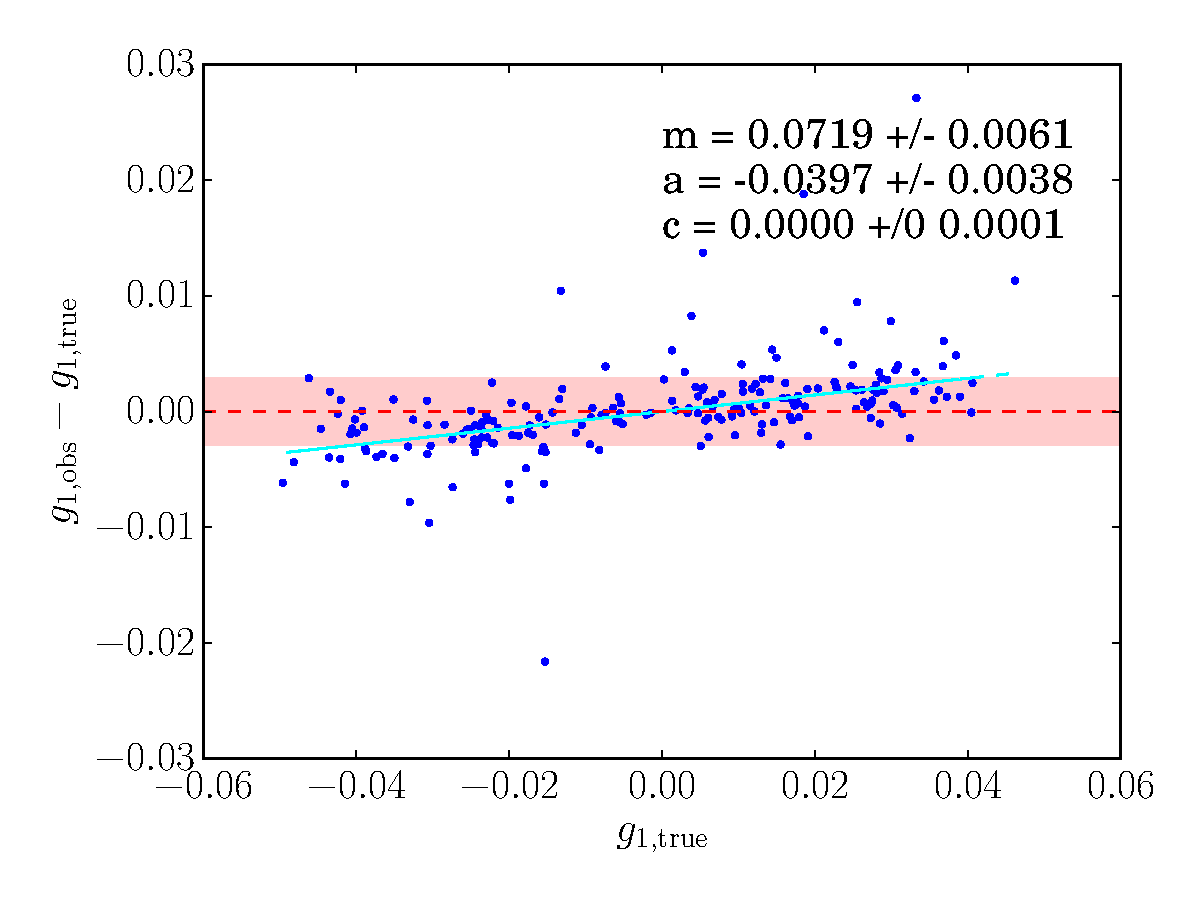
\includegraphics[width=0.46\linewidth]{./Plots/m1-no_corrections-regauss.pdf}
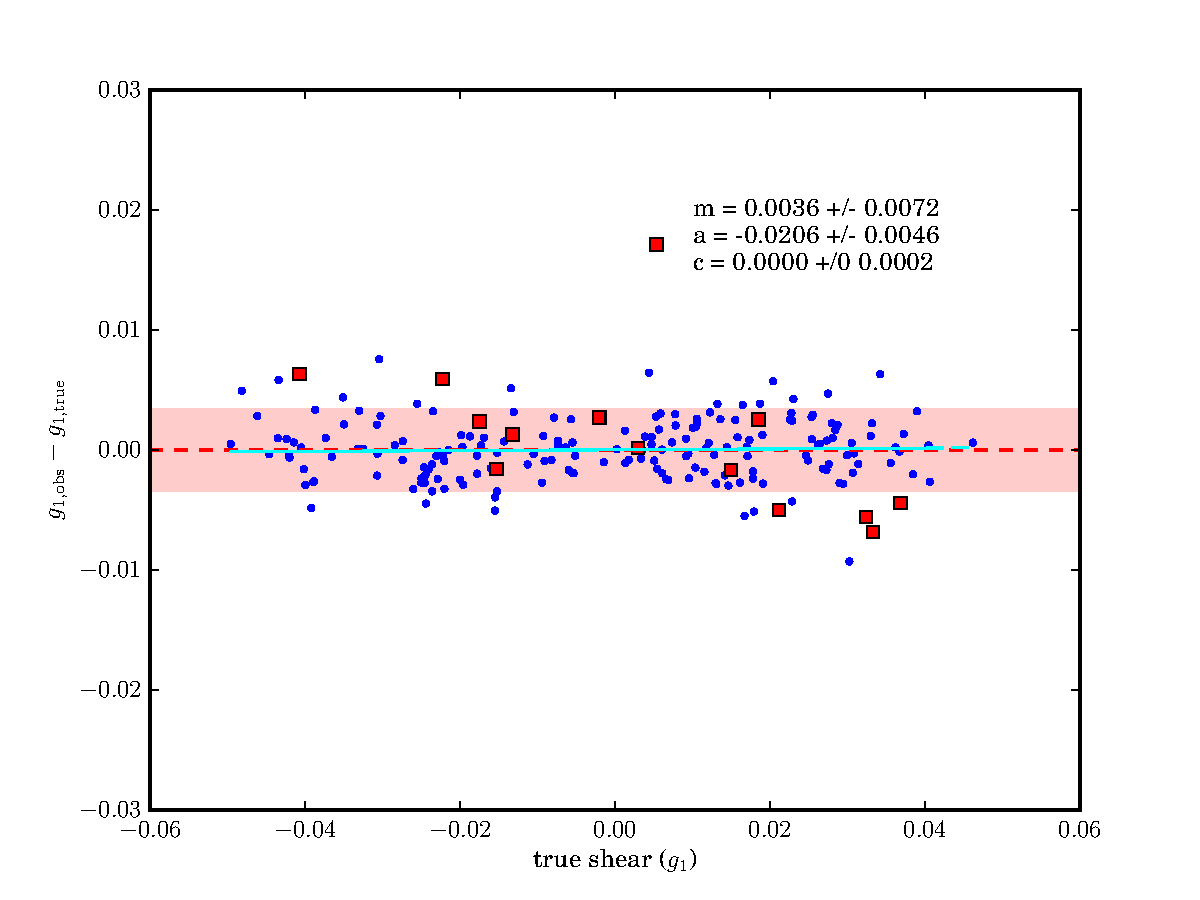
\includegraphics[width=0.46\linewidth]{./Plots/m1-regauss-opt-shear_plots.pdf}\\
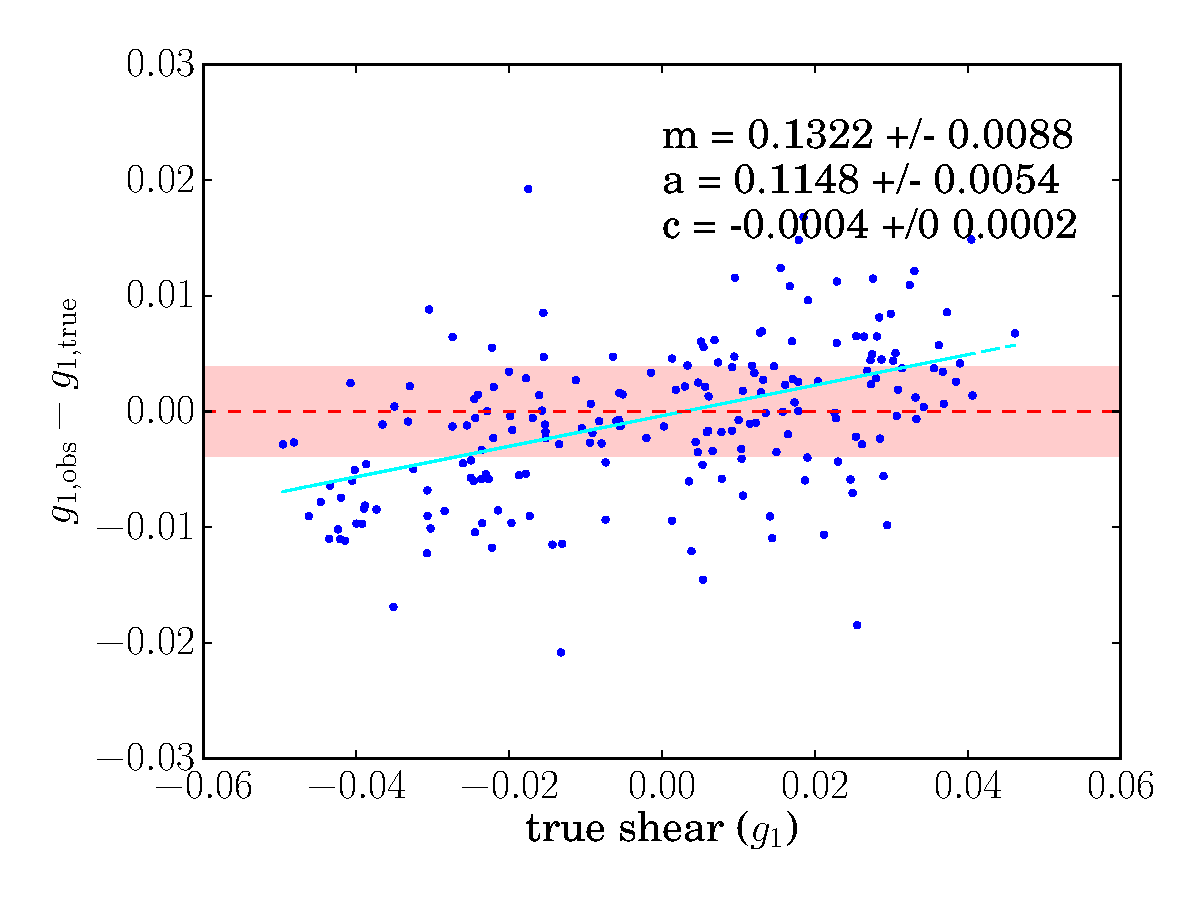
\includegraphics[width=0.46\linewidth]{./Plots/m1-no_corrections-ksb.pdf}
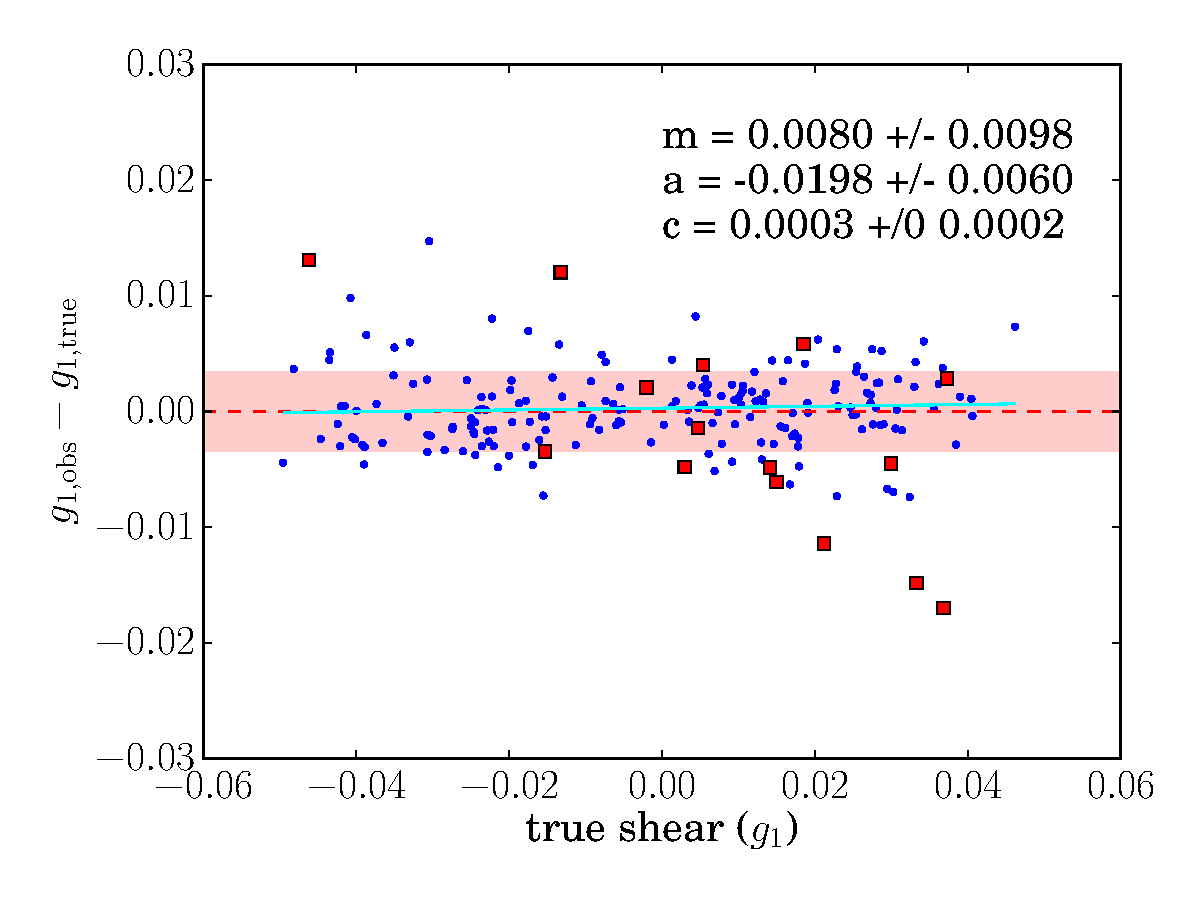
\includegraphics[width=0.46\linewidth]{./Plots/m1-ksb-opt-shear_plots.pdf}\\
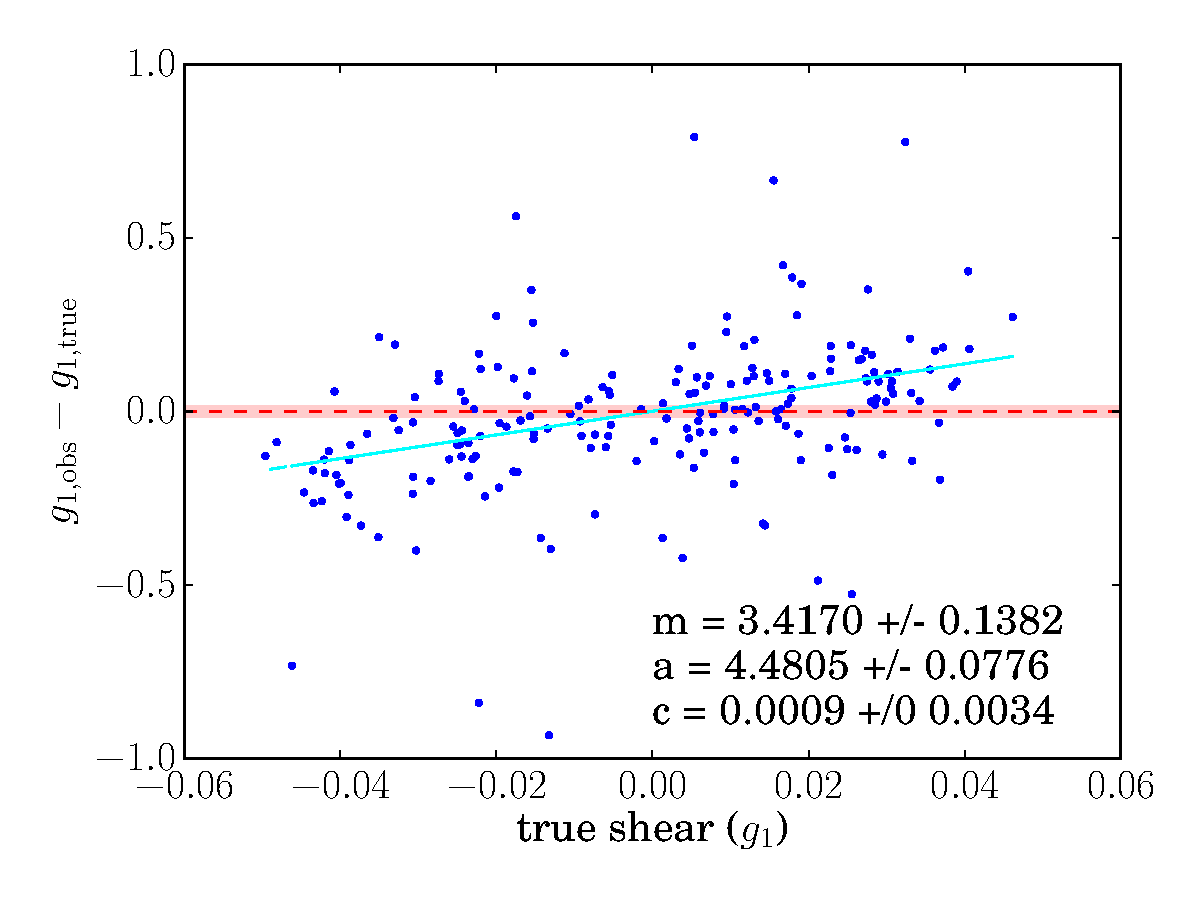
\includegraphics[width=0.46\linewidth]{./Plots/m1-no_corrections-moments.pdf}
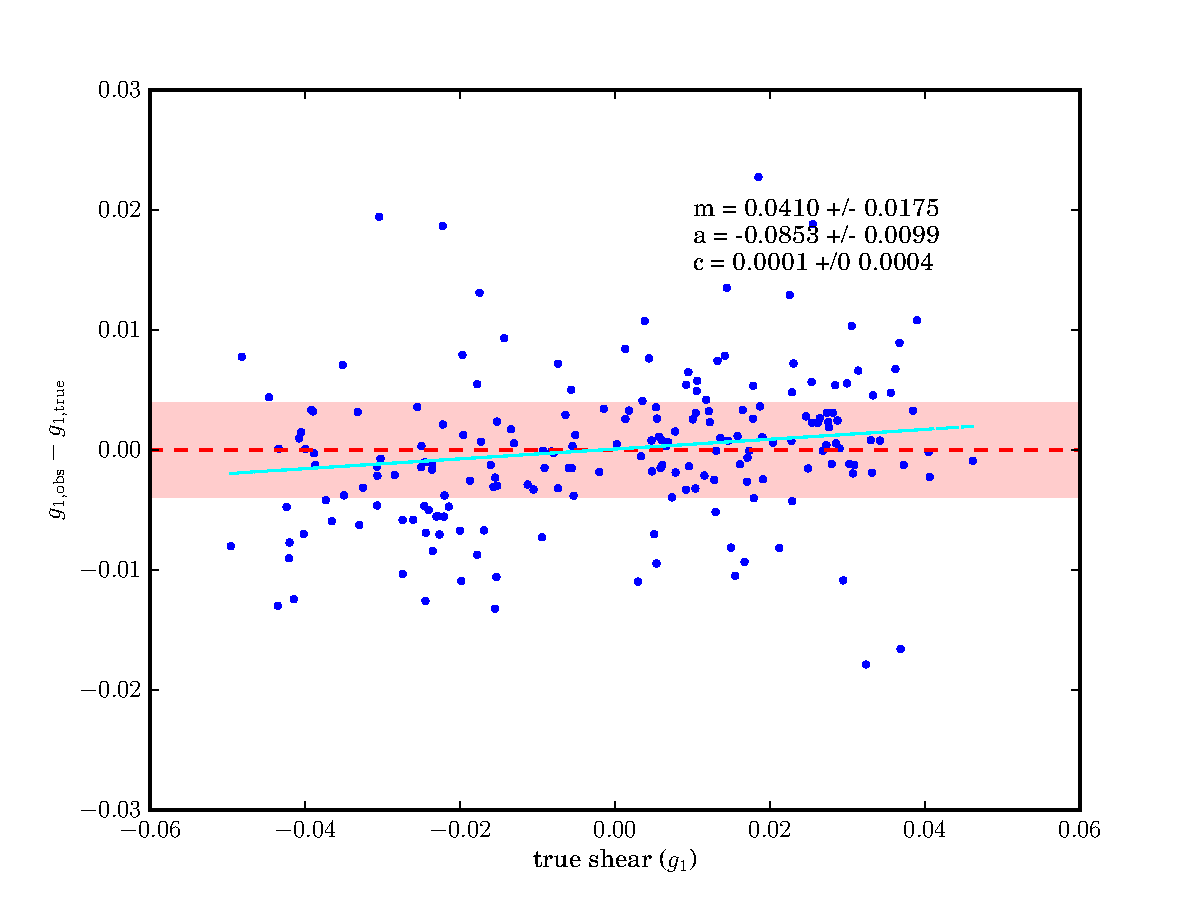
\includegraphics[width=0.46\linewidth]{./Plots/m1-moments-opt-shear_plots.pdf}
\end{center}
\caption{Shear calibration bias $m_1$ {\it before} ({\bf left}) and
  {\it after} {\bf right} metacalibration for the regaussianization
  ({\bf top}), KSB ({\bf middle}), and Linear Moments ({\bf bottom})
  algorithms on the CGC branch. The shaded region covers the same
  vertical range in each panel.  Points excluded by the log-likelihood
  cut are marked with red squares.}
\label{fig:m_comparison}
\end{figure*}



%\begin{figure*}[t]
%\begin{center}
%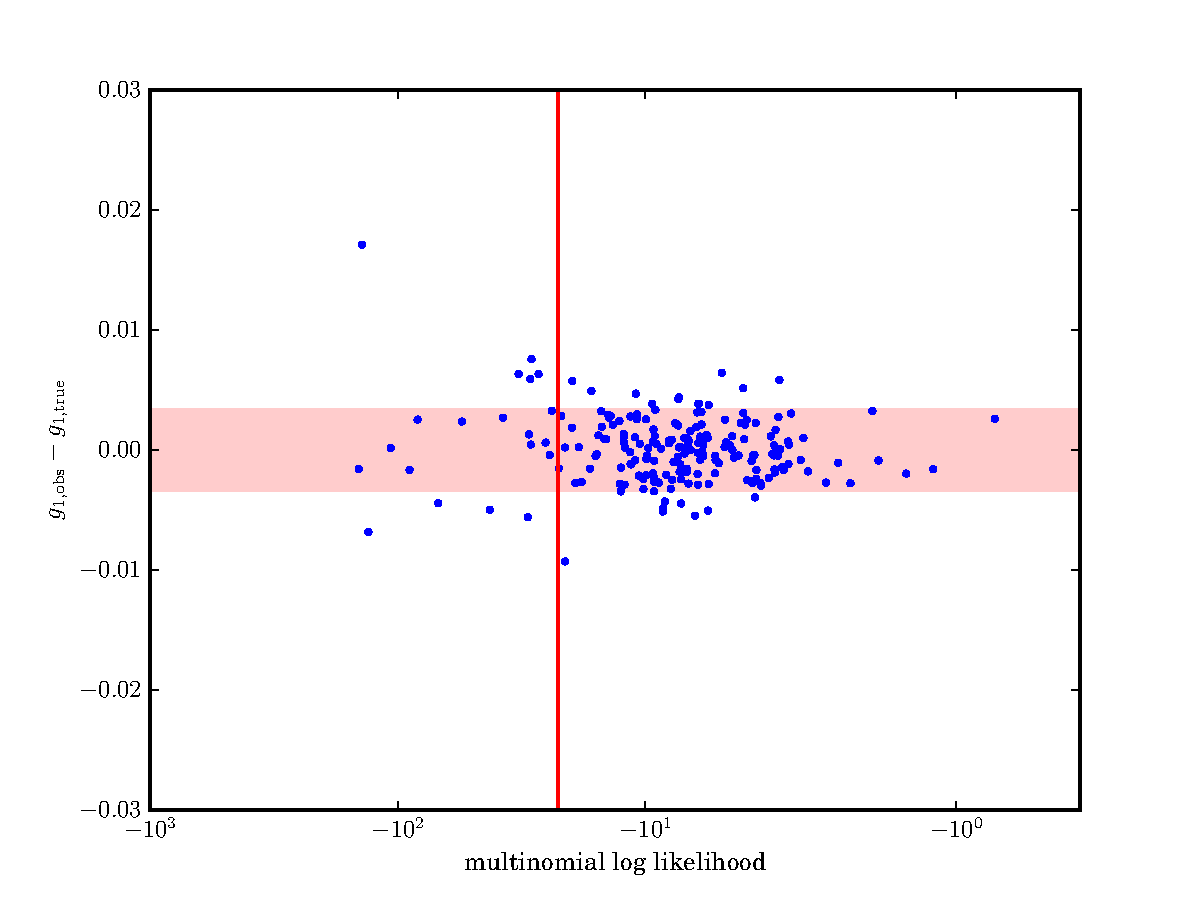
\includegraphics[width=0.48\linewidth]{./Plots/logL1-regauss-opt-shear_plots.pdf}
%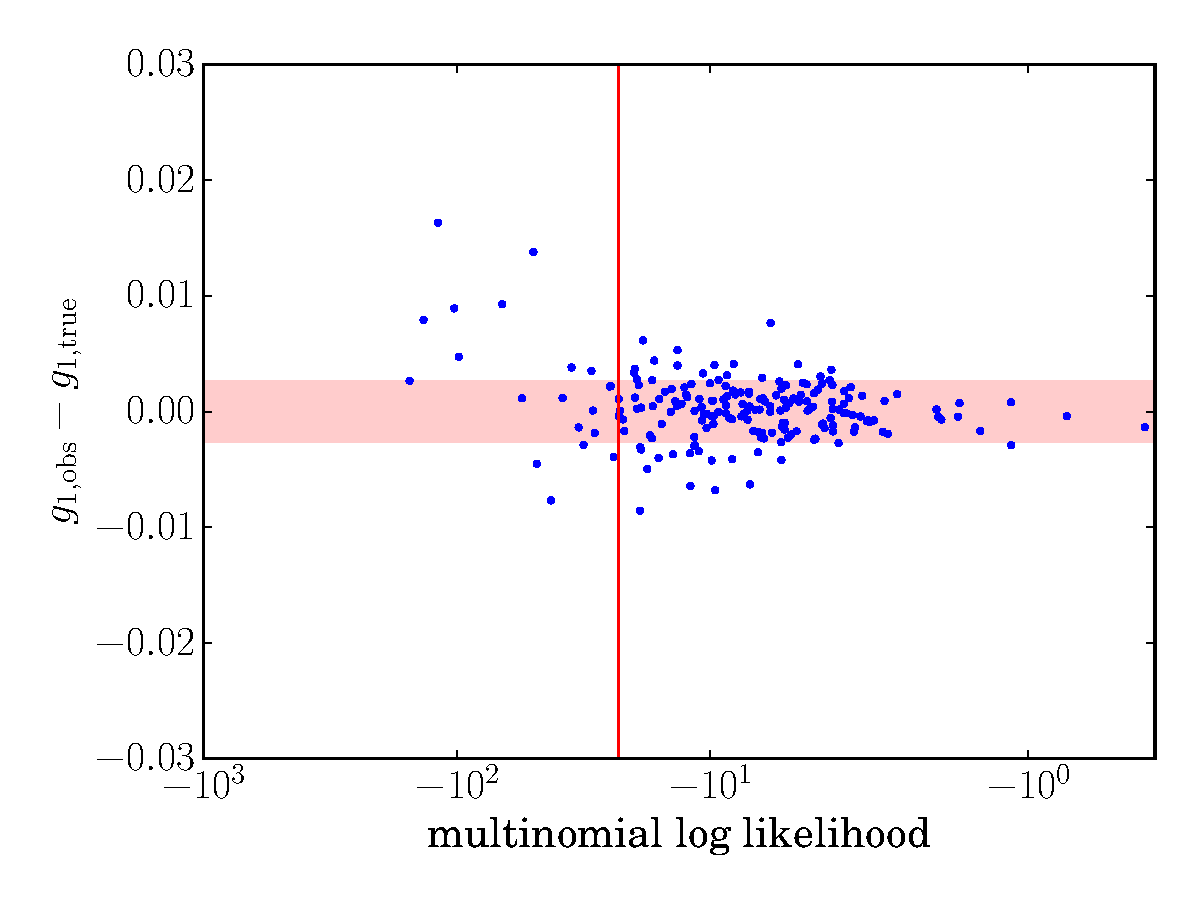
\includegraphics[width=0.48\linewidth]{./Plots/logL1-rgc-regauss-opt-shear_plots.pdf}
%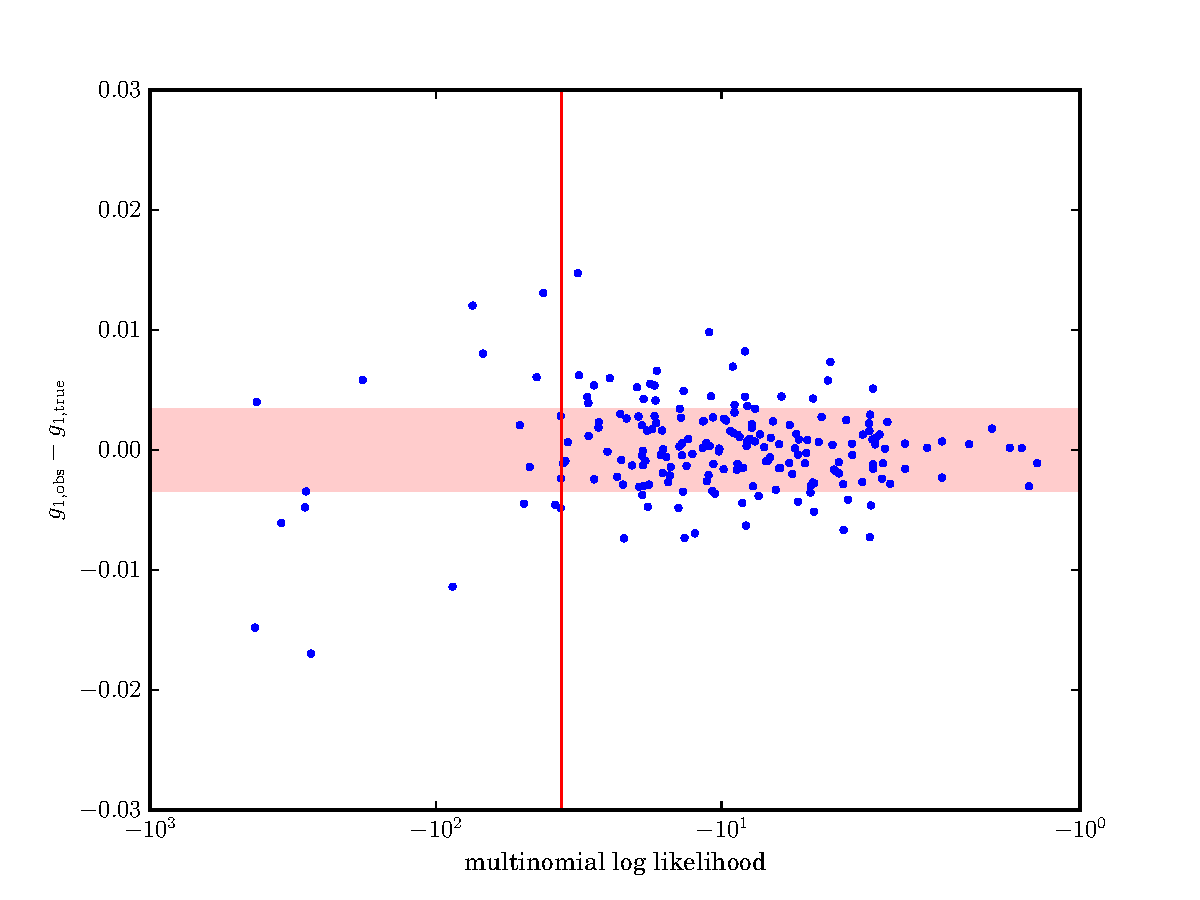
\includegraphics[width=0.48\linewidth]{./Plots/logL1-ksb-opt-shear_plots.pdf}
%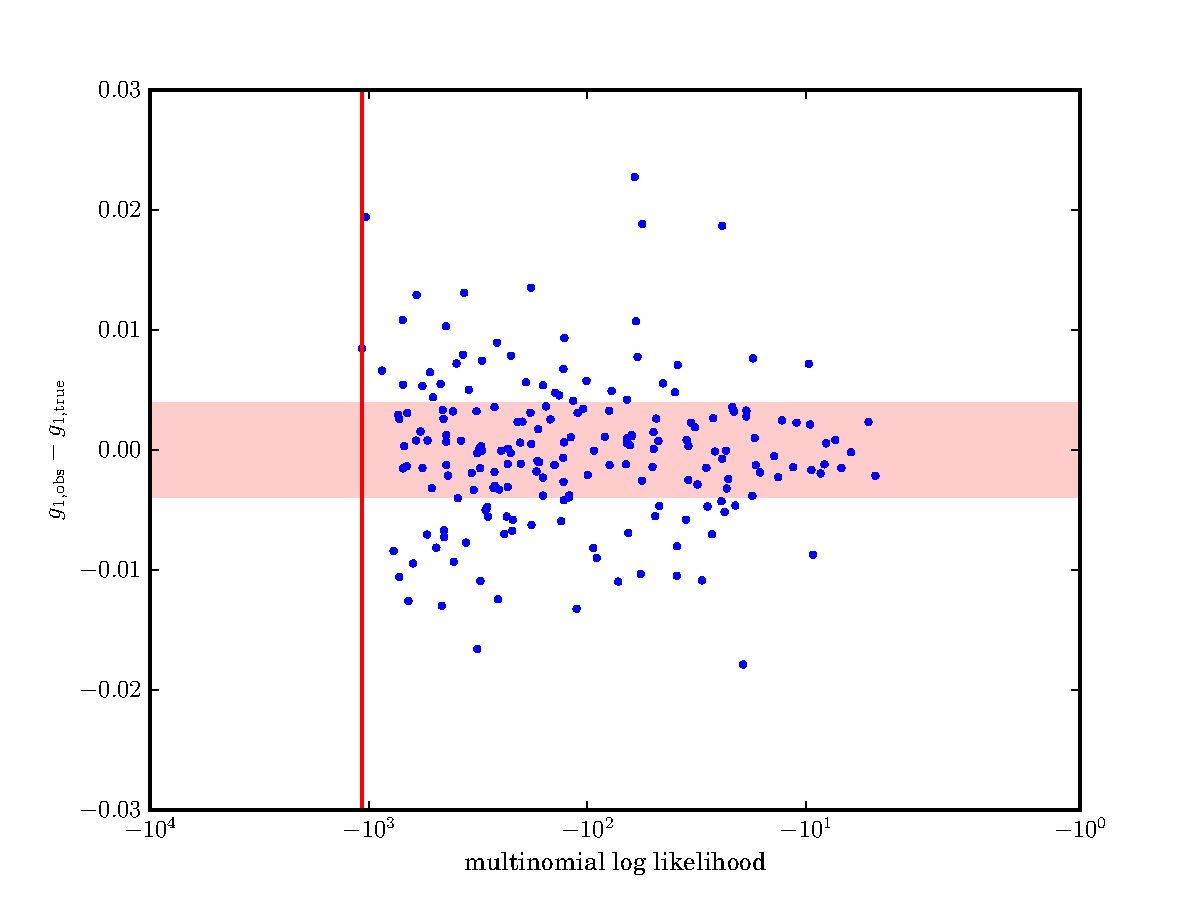
\includegraphics[width=0.48\linewidth]{./Plots/logL1-moments-opt-shear_plots.pdf}
%\end{center}
%\caption{log-likelihoods used to rank-order fields for applying
% cuts. Vertical red line indicates location of $20\%$ $\log L$
% cut. This metric tends to be a reliable indicator whether
% the inference procedure will fail. Clockwise from the top-left
% panel: CGC-regauss, RGC-regauss, CGC-moments, and CGC-KSB.}
%\end{figure*}

%\begin{figure*}[t]
%\begin{center}
%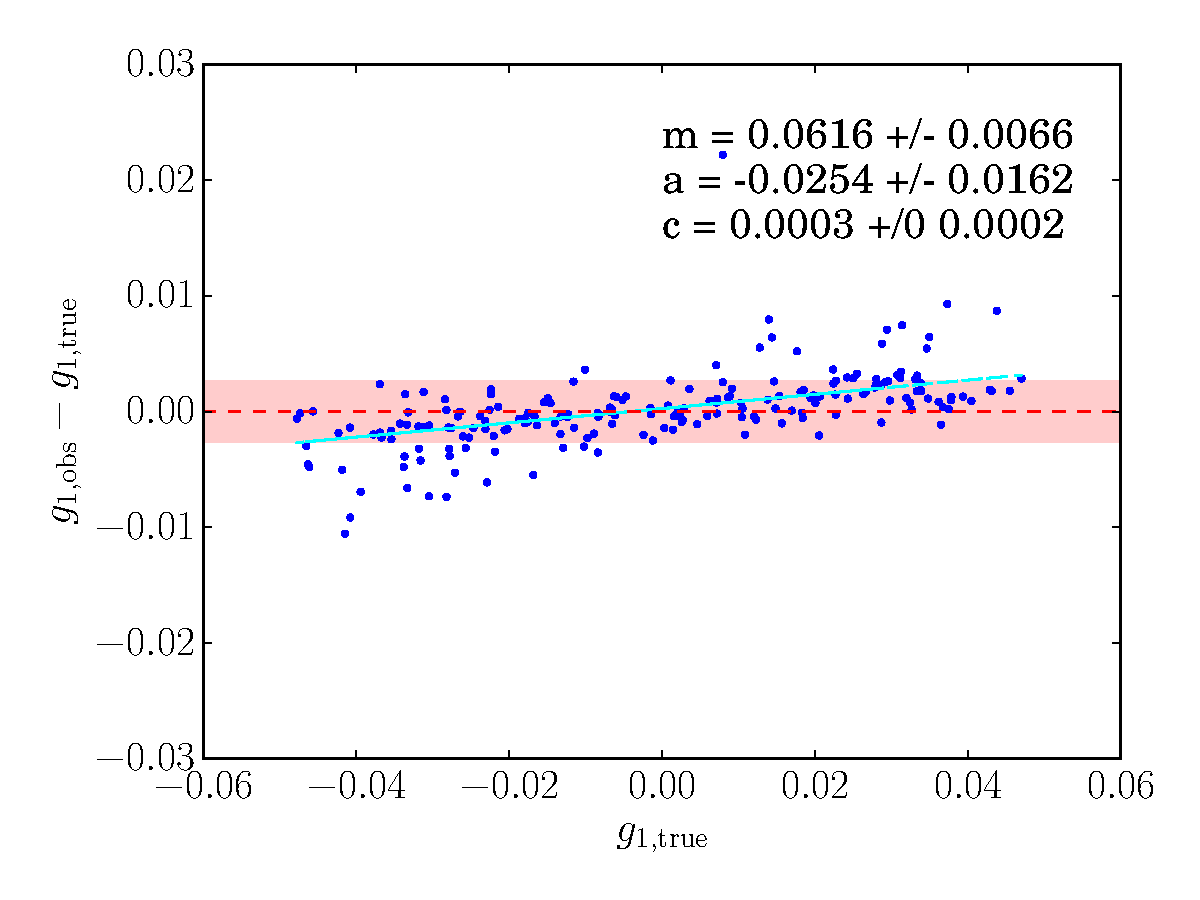
\includegraphics[width=0.48\linewidth]{./Plots/m1-no_corrections-rgc-fixedaber-regauss.pdf}
%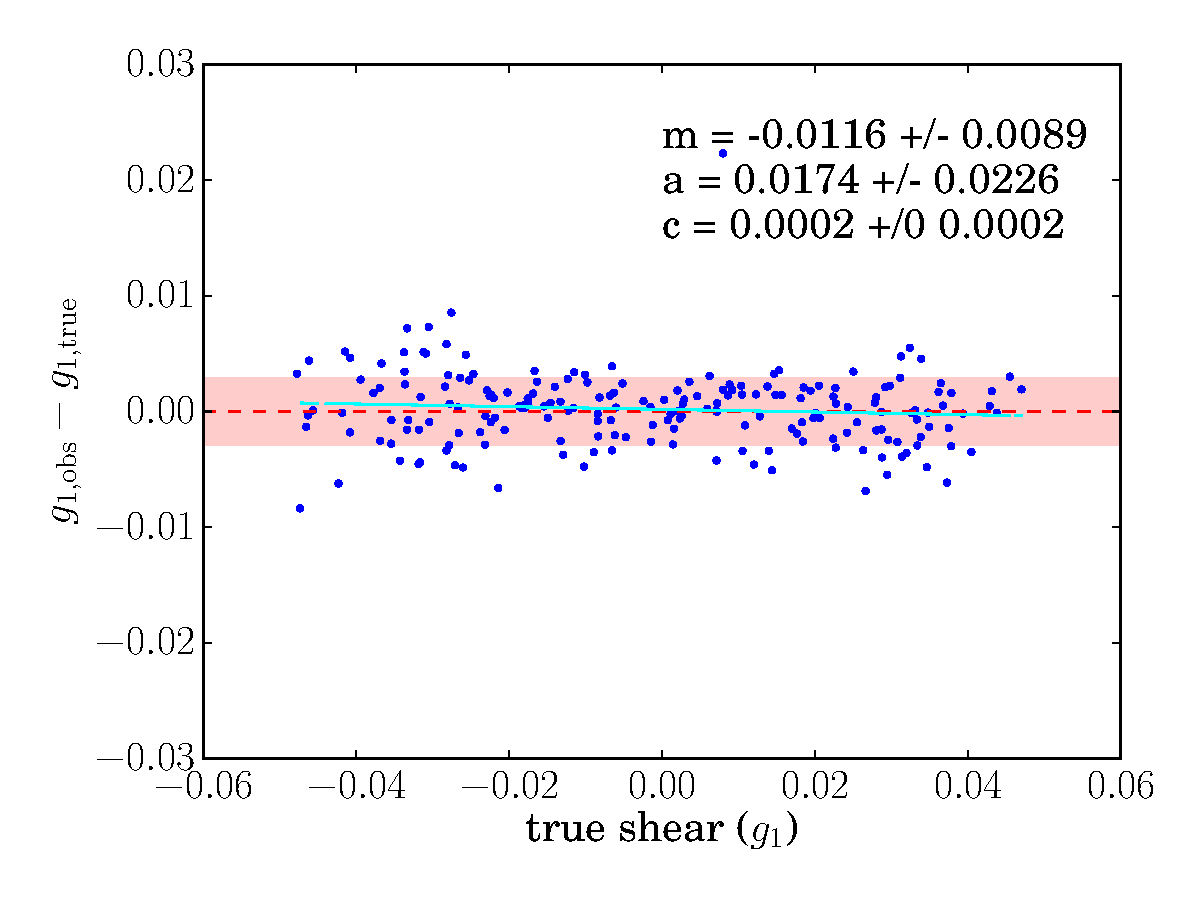
\includegraphics[width=0.48\linewidth]{./Plots/m1-rgc-fixedaber-regauss-opt-shear_plots.pdf}
%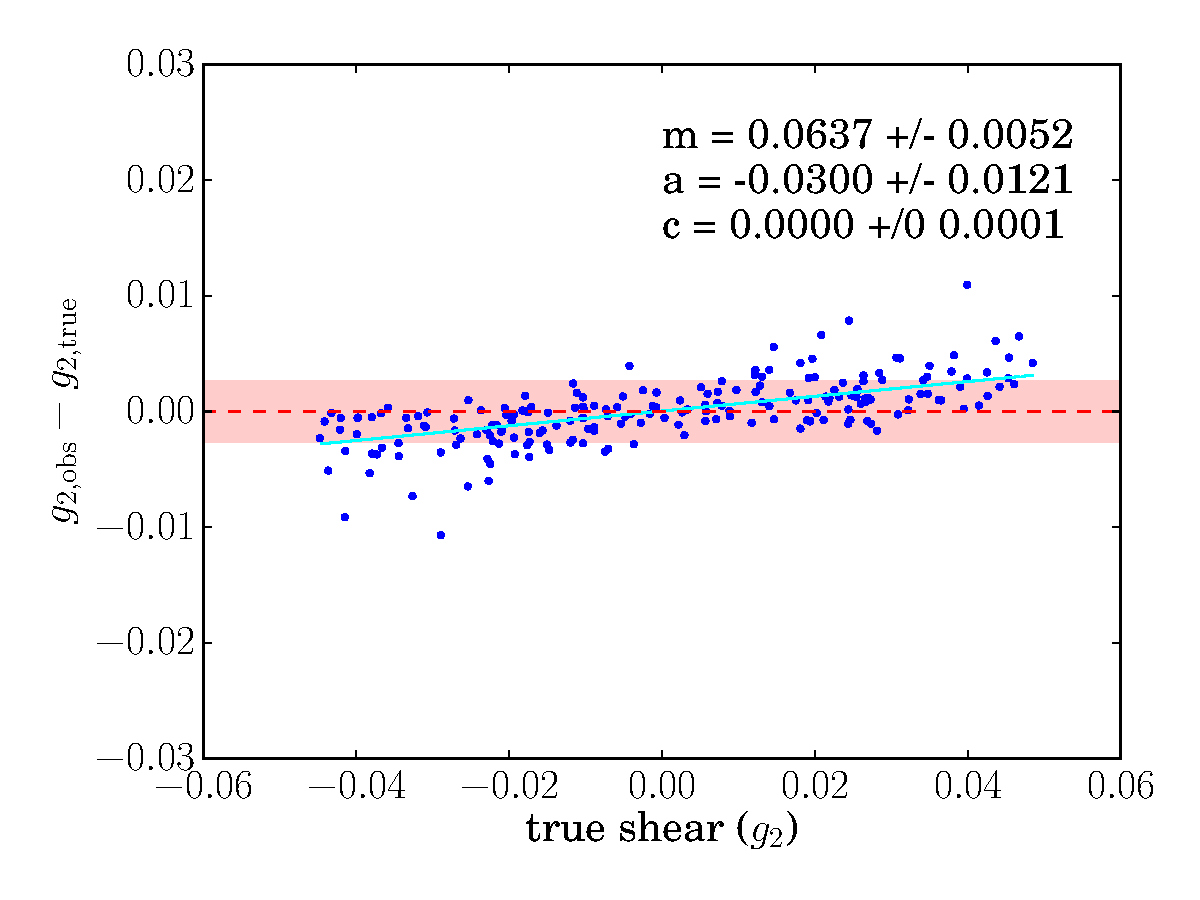
\includegraphics[width=0.48\linewidth]{./Plots/m2-no_corrections-rgc-fixedaber-regauss.pdf}
%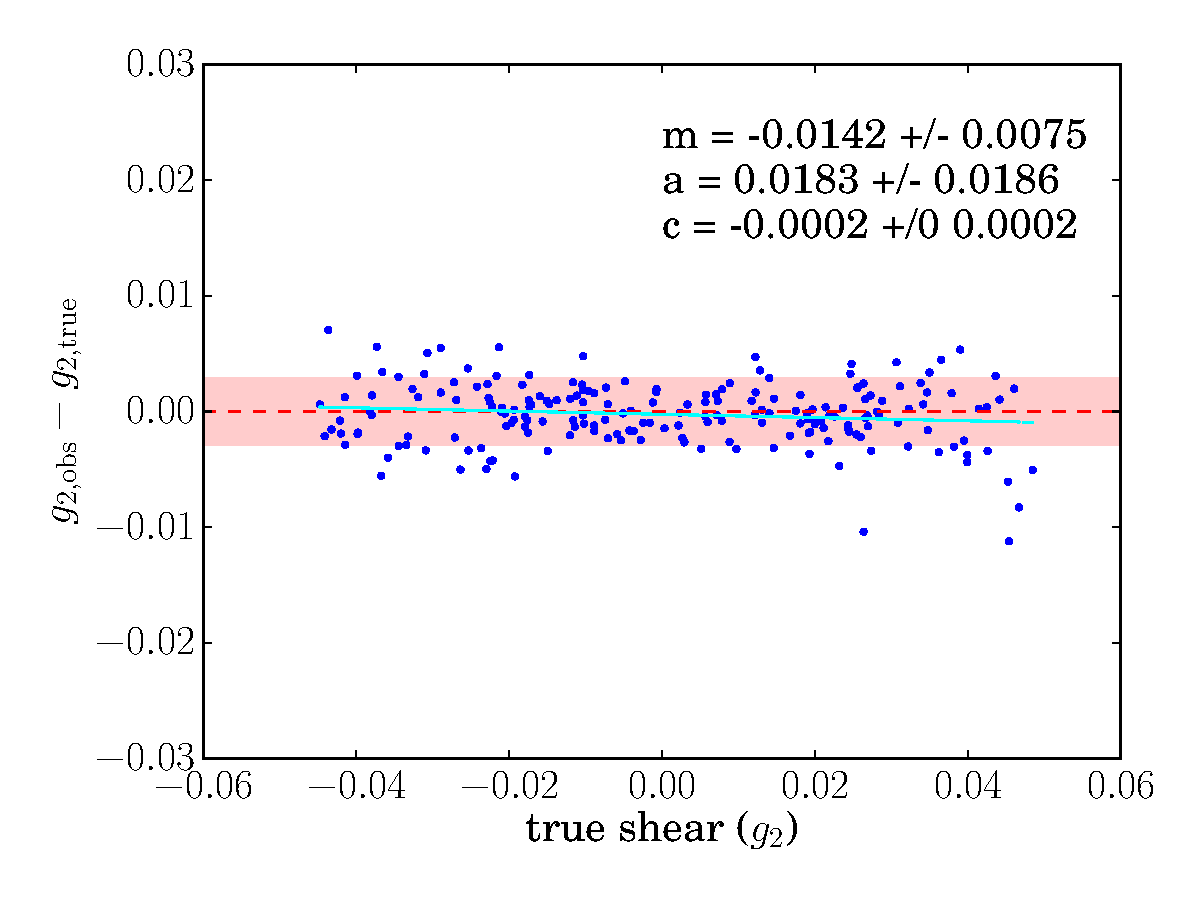
\includegraphics[width=0.48\linewidth]{./Plots/m2-rgc-fixedaber-regauss-opt-shear_plots.pdf}
%\end{center}
%\caption{Multiplicative calibration results for the rgc-fixedaber
% branch.}
%\end{figure*}

\begin{figure}
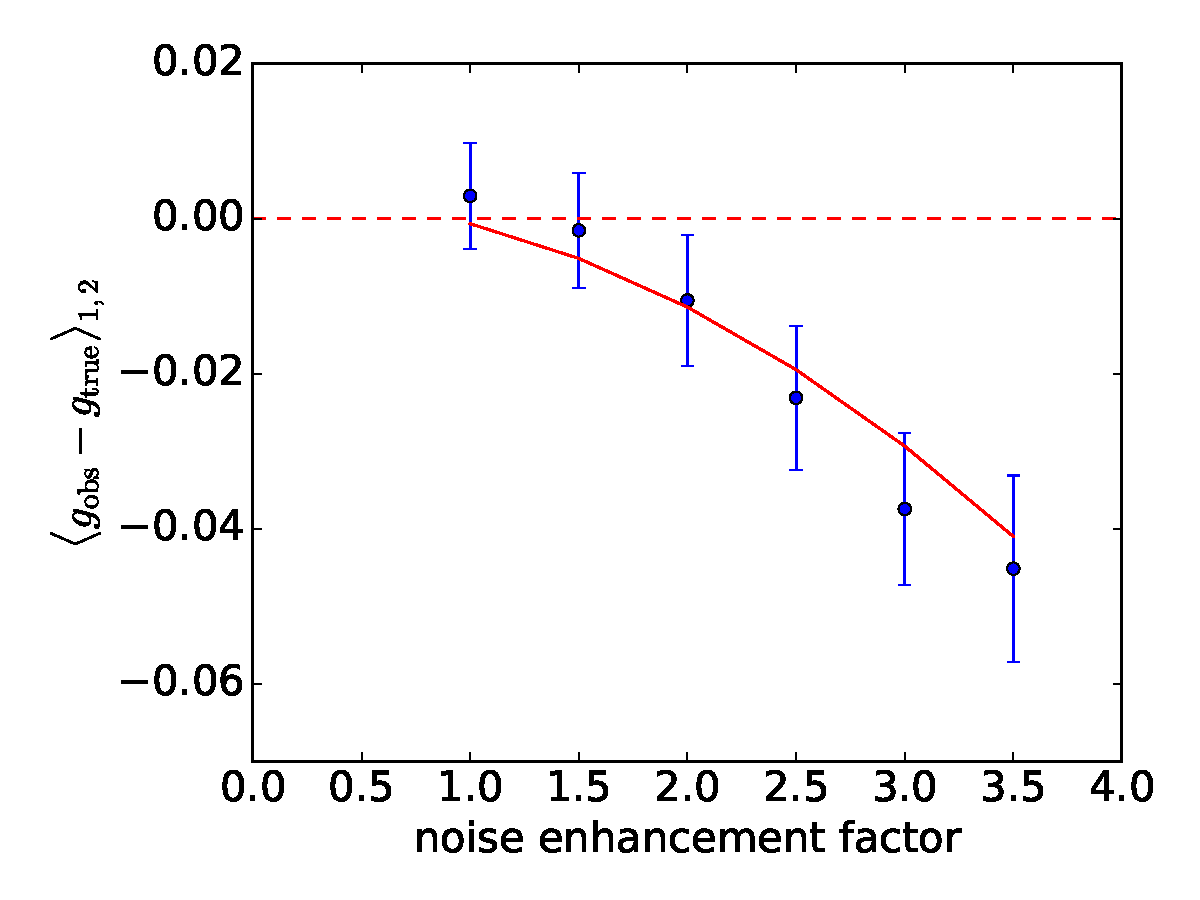
\includegraphics[width=\columnwidth]{./Plots/noise_bias_test.pdf}
\caption{Effects of introducting additional noise. Points with errors
  correspond to multiplicative shear calibration bias in the
  control-ground-constant branch when additional noise is added. The
  noise enhancement factor corresponds to the factor by which the
  noise in each galaxy image is increased relative to the fiducial
  GREAT3 simulations. The solid red line shows the expected power-law scaling
  resulting from correlated noise bias, with a normalization fixed to
  the measured calibration biases.}
\label{fig:noise_bias}
\end{figure}


\begin{figure}
\begin{center}
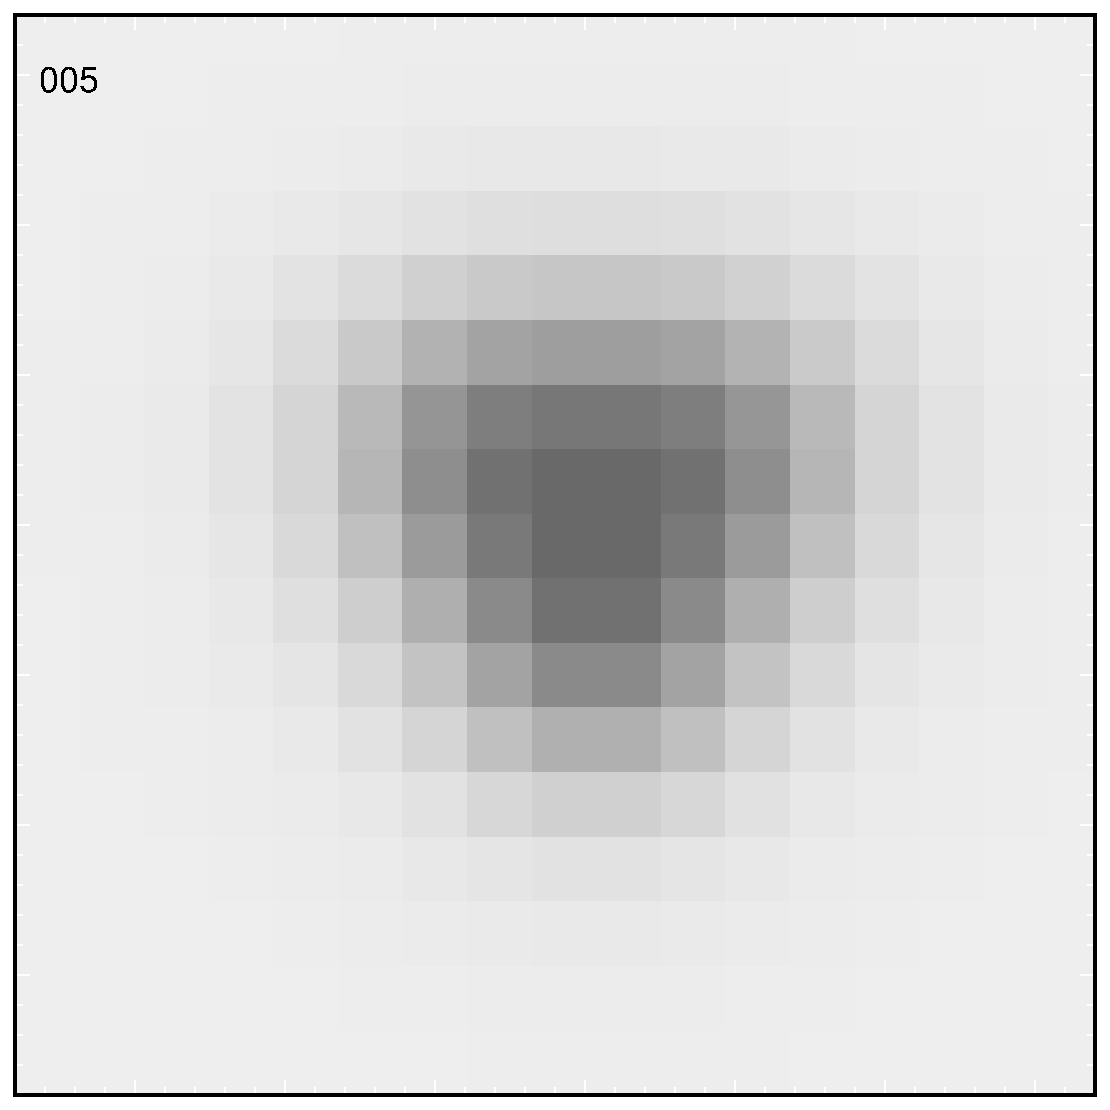
\includegraphics[width=0.8\columnwidth]{../Plots/rgc_fixedaber_psf_005.pdf}
\end{center}
\caption{Example of a PSF in one of the simulations with fixed, large aberrations.  The most obvious
feature in this case is the trefoil, which gives rise to the triangular shape. \label{fig:trefoil}}
\end{figure}

\begin{figure*}
\begin{center}
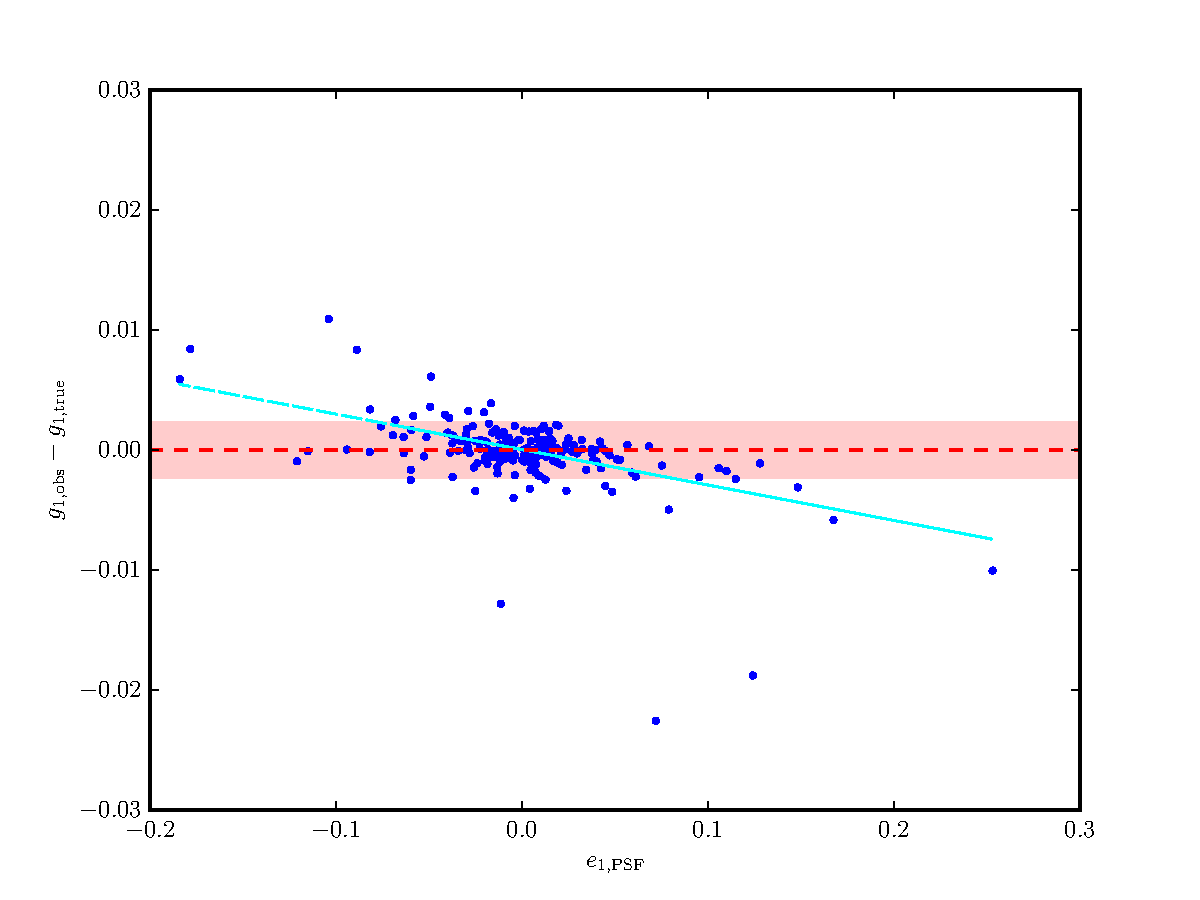
\includegraphics[width=0.4\linewidth]{./Plots/psf_e1-no_corrections-rgc-regauss.pdf}
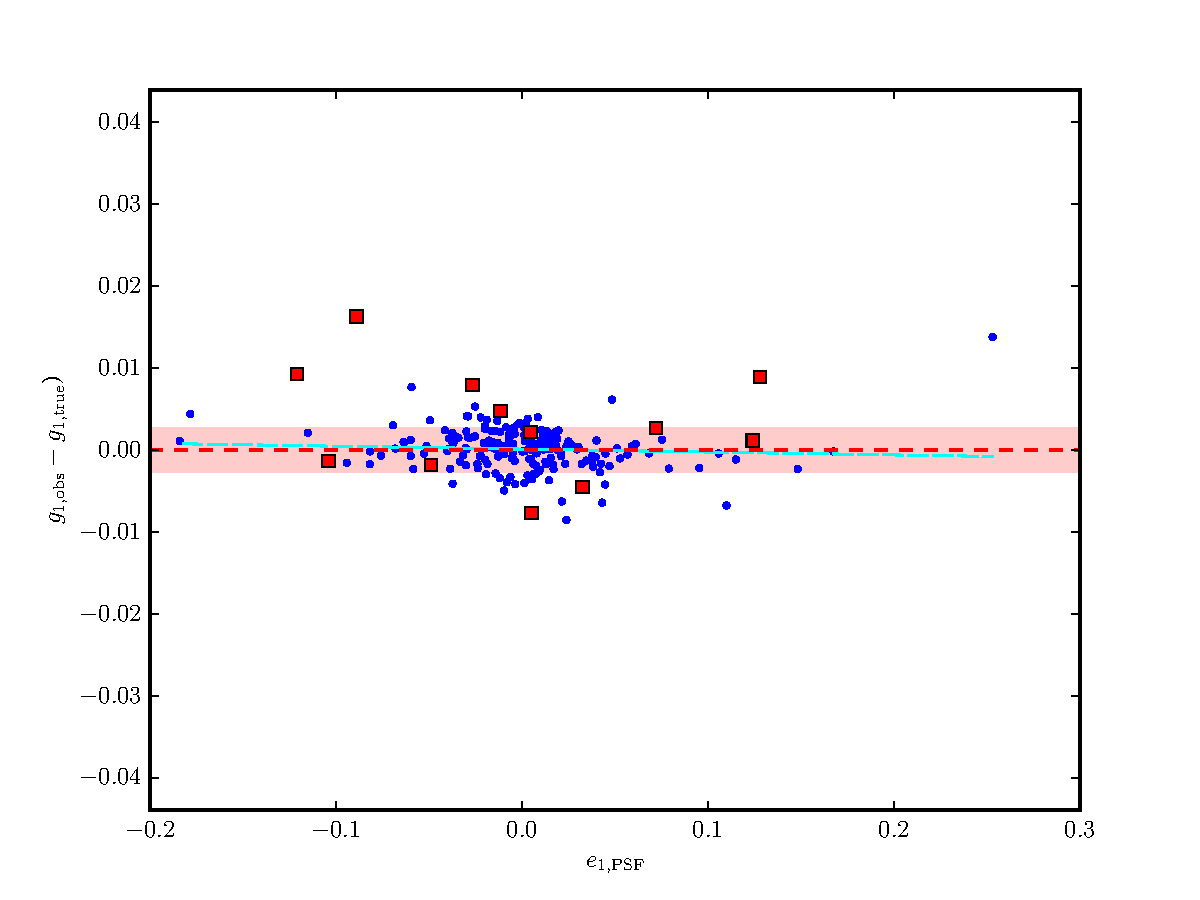
\includegraphics[width=0.4\linewidth]{./Plots/psf_e1-rgc-regauss-opt-shear_plots.pdf}
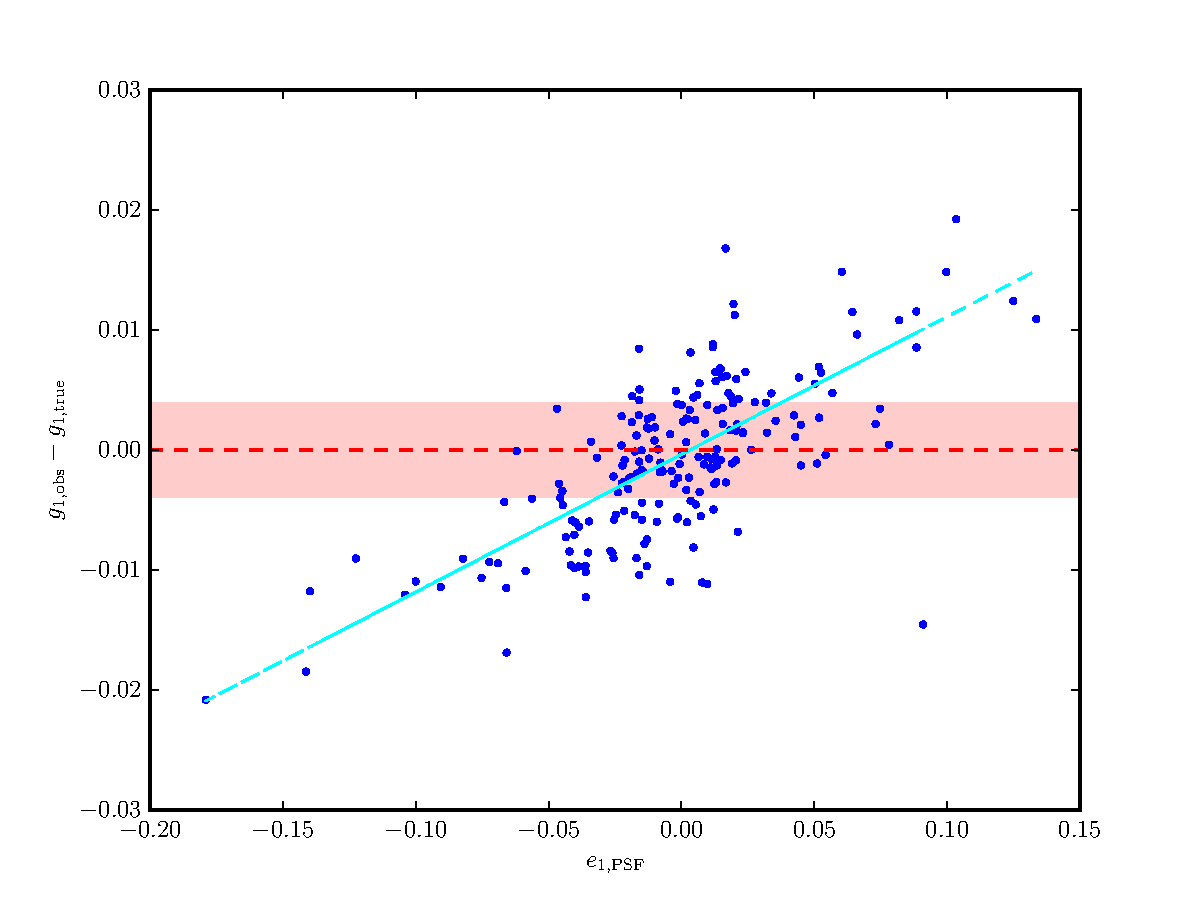
\includegraphics[width=0.4\linewidth]{./Plots/psf_e1-no_corrections-ksb.pdf}
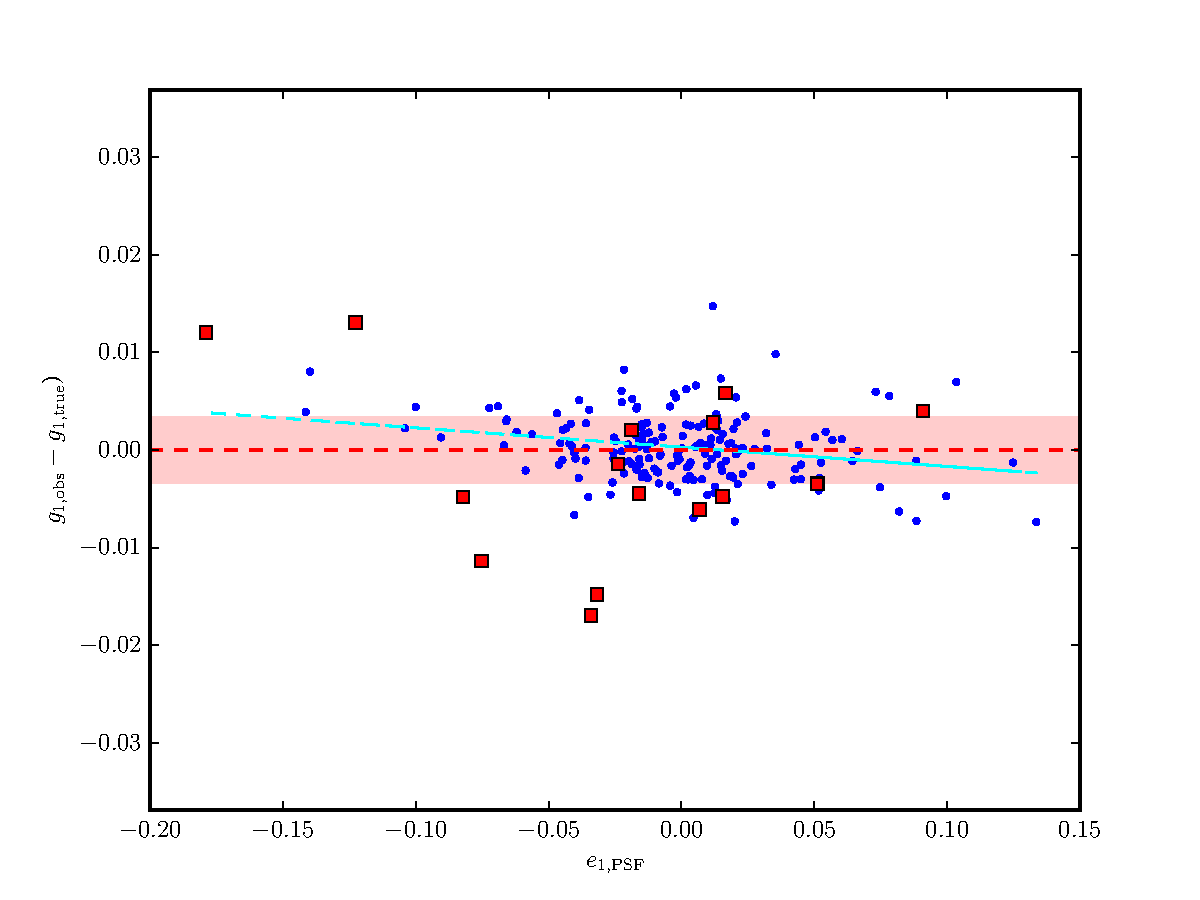
\includegraphics[width=0.4\linewidth]{./Plots/psf_e1-ksb-opt-shear_plots.pdf}
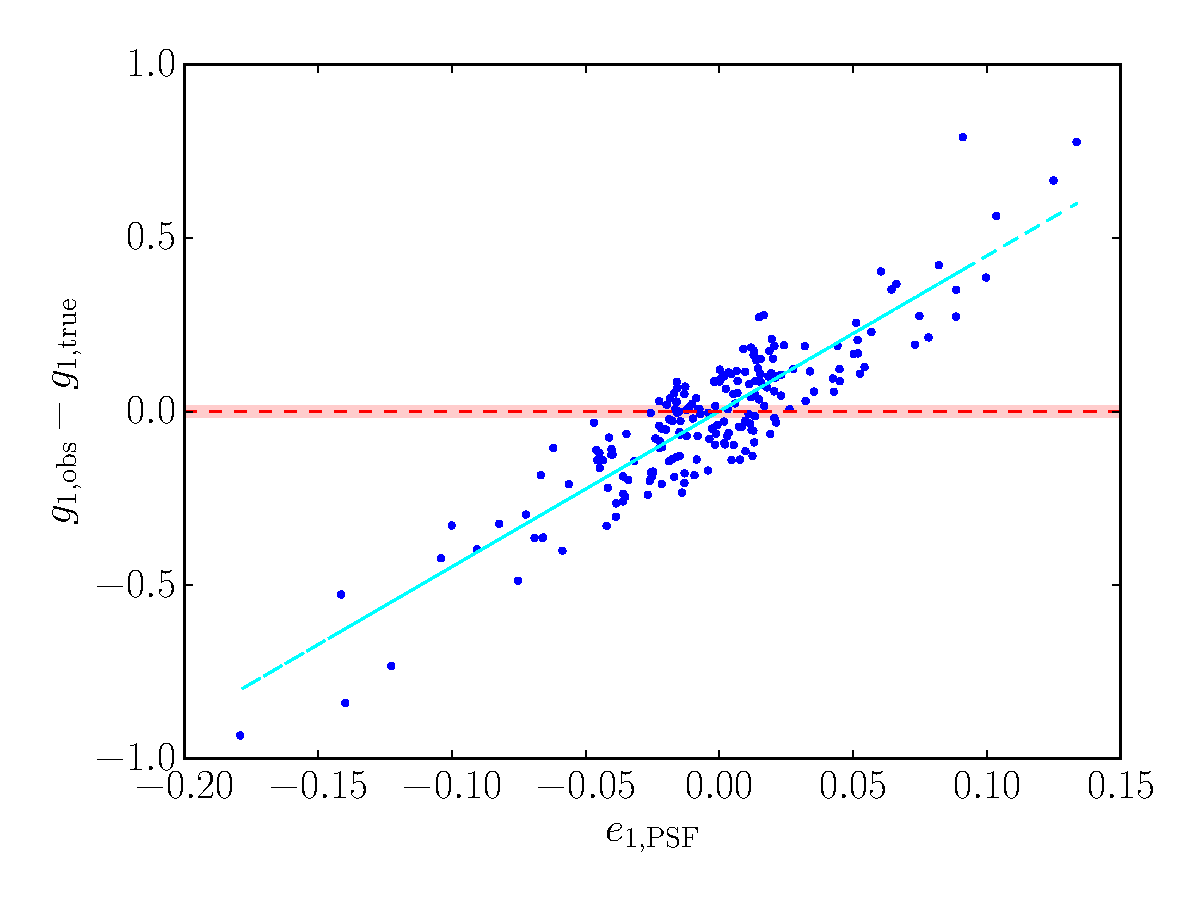
\includegraphics[width=0.4\linewidth]{./Plots/psf_e1-no_corrections-moments.pdf}
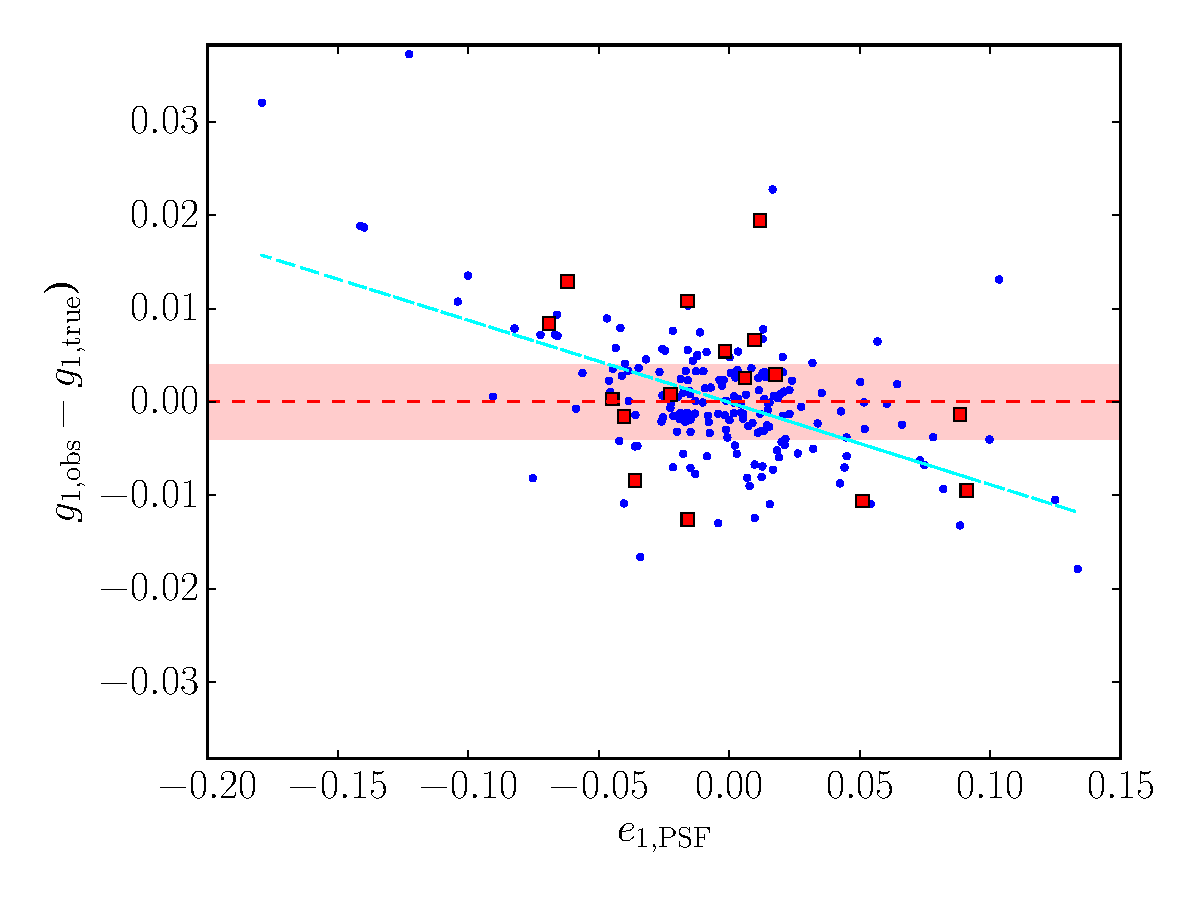
\includegraphics[width=0.4\linewidth]{./Plots/psf_e1-moments-opt-shear_plots.pdf}
\end{center}
\caption{Effects of the metacalibration alogorithm applied to PSF
  correction. {\bf Left} panels show the relationship between measured
  shear and PSF ellipticity before correction, and {\bf right} panels
  show the same trends afterwards. Note that the shaded horizontal
  band covers the same vertical range in each panel.  \\
  Simulation branch/algorithm pairs shown in order from {\bf top} to
  {\bf bottom} are RGC-regauss, CGC-KSB, and CGC-moments. The
  combination of the metacalibration algorithm with our
  maximum-likelihood averaging procedure makes accurate corrections
  when the PSF ellipticities are small or comparable to the magnitude
  of the shear signal. It is clear that a large fraction of the trend
  remaining after correction is driven by high-PSF-ellipticity outlier
  fields, which would typically not pass the image quality
  requirements in a realistic experiment.}
\label{fig:psf_trends}
\end{figure*}

\section{Applicability to real data}
Several implementation issues need to be solved before this method can
be deployed on real survey data. We have made no attempt to deal with
the effects of masked pixels or blending, and while it seems clear
that our proposed algorithm has the potential to deal with selection
biases, we have not demonstrated that capability here. We have also
demonstrated the presence of a calibration bias which scales with the
variance of the pixel noise, which may be a result of the correlations
imposed on the noise field during the construction of the
counterfactual image.

In this work, we have attempted to remove PSF systematics by measuring
the response of the shape measure to PSF ellipticity. There is no
guarantee, however, that the PSF ellipticity is the correct parameter
to use for this detrending. In a realistic measurement, it would be
best to first determine which modes of PSF variation are most likely
to impact the chosen shape measure, and then use the image
modification and detrending technique described here to remove those
effects in the data.

Finally, our shear inference procedure is designed to extract the mean
shear from a constant-shear field. While this procedure may be
applicable to galaxy-galaxy lensing (i.e., projecting the shapes onto
the tangent to the appropriate lens), it is not suitable for
measurements like cosmic shear that typically rely on second or higher
moments of the shear field. While a similar histogram estimation
procedure could be implemented to model the responsivity of the
distribution of ellipticity products (as would be needed for two-point
shear correlation functions), we leave design and implementation of
this generalization to for future work.

At the time of this writing, metacalibration is being actively adapted
to realistic measurements in the Dark Energy Survey. Follow-up work
(Sheldon et al.\ 2016) will demonstrate algorithmic improvements that
allow this technique to be used on Dark Energy Survey data with
state-of-the-art shear estimation algorithms.



\section{Conclusions}
We have proposed and implemented the first method for self-calibration
of shear measurements that does not rely on external data or
simulations for shear calibration. Our method can be wrapped around
any sufficiently well-behaved shape measurement algorithm.  We use
GREAT3 and related simulations to demonstrate that metacalibration
reduces or eliminates shear calibration biases across a variety of
galaxy morphologies, PSF properties, and for several otherwise biased
shape measurement algorithms. We have argued that our technique works
because it takes advantage of the fundamental linearity of
astronomical images in the shear signal, most astronomical
imaging, in combination with the fact that the effects of
shear on an image with a known PSF are model-independent.

Those cases we have examined where the initial biases are large or not
linear are not completely corrected by our linear detrending scheme,
though in every case we have studied the algorithm appears to
substantially improve biases resulting from faulty PSF correction and
shear miscalibration. Even the nearly information-free linear moments
algorithm appears to be calibrated by our procedure to a level
superior to uncorrected KSB, a widely used traditional shear
estimation algorithm.

We expect future work to extend this method to deal with the
complexities inherent in real data.


\begin{figure*}
\makebox[\textwidth][c]{
\begin{tabular}{l  c |cc | cc |cc }
\hline
branch & algorithm  &  $m_1\times1000$ & $m_2\times1000$  & $a_1\times1000$ & $a_2\times1000$ &  $c_1\times1000$ & $c_2\times1000$ \\
\hline
\hline
CGC & regauss (MC)  & $3.6 \pm 7.2$ & $2.3\pm 6.4$ & $-20.6\pm4.6$ & $-19.4\pm3.6$ &  $0.0\pm.2$ & $0.1\pm0.2$ \\
CGC & regauss  &  $71.9\pm6.1$ & $65.5\pm4.9$  & $-39.7\pm3.8$ & $-43.9\pm2.9$ &  $0.0\pm0.1$ & $0.0\pm0.1$ \\
%CGC & regauss-noisy (MC) & $-15.0\pm 8.9$ & $3.7\pm7.9$ & $-24.5\pm5.7$ & $-19.7\pm4.5$ & $-0.1\pm0.2$ & $-0.1\pm0.2$\\
%CGC & regauss-noisy & $117.2 \pm  7.7$ & $105.2\pm6.6 $ & $40.2\pm4.9$ & $-48.4\pm4.1$ & $0.2\pm0.2$ & $-0.1\pm0.2$ \\
CGC & ksb (MC)  &  $8.0\pm9.8$ & $-17.0\pm8.7$  & $-19.8\pm6.0$ & $-9.2\pm5.0$ &  $0.3\pm0.2$ & $-0.2\pm0.2$ \\
CGC & ksb  &  $132.2\pm8.8$ & $145.5\pm10.4$  & $114.8\pm5.4$ & $109.6\pm6.1$ &  $-0.4\pm0.2$ & $0.0\pm.3$ \\
CGC & moments (MC) & $37.1\pm17.3$ & $45.9\pm18.4$ & $-88.0\pm9.9$ & $-87.7\pm9.5$ & $0.1\pm0.4$ & $-0.2\pm0.5$\\
CGC & moments & $3417.0\pm138.2$ & $3223.8\pm173.1$ & $4480.5\pm77.6$ & $4604.4\pm88.8$ & $0.9\pm3.4$ & $-0.8\pm4.6$ \\
RGC & regauss (MC) &  $-5.3\pm7.8$ & $6.1\pm6.6$  & $3.6\pm4.0$ & $-3.1\pm3.7$ &  $0.1\pm0.2$ & $0.1\pm0.2$ \\
RGC & regauss &  $30.4\pm5.2$ & $24.9\pm5.0$  & $-29.5\pm2.8$ & $-18.6\pm2.8$ &  $0.0\pm0.1$ & $0.2\pm0.1$ \\
CGC-Noaber & regauss (MC)  &  $-7.4\pm6.9$ & $6.1\pm6.4$  & $-33.9\pm12.7$ & $-23.7\pm11.2$ &  $0.1\pm0.2$ & $0.1\pm0.2$ \\
CGC-Noaber & regauss  &  $40.7\pm2.9$ & $-43.9\pm2.9$  & $-27.4\pm5.2$ & $-26.5\pm5.0$ &  $0.1\pm0.1$ & $0.1\pm0.1$ \\
RGC-Noaber & regauss (MC)&  $7.5\pm5.0$ & $14.0\pm4.8$  & $-18.8\pm9.6$ & $-10.8\pm9.1$ &  $0.0\pm0.1$ & $0.0\pm0.1$ \\
RGC-Noaber & regauss &  $16.4\pm3.0$ & $17.4\pm3.4$  & $2.2\pm5.8$ & $2.5\pm6.4$ &  $0.2\pm0.1$ & $0.0\pm0.1$ \\
RGC-FixedAber & regauss (MC) &  $-4.7\pm8.9$ & $6.0\pm7.2$  & $-15.4\pm22.1$ & $-16.0\pm17.5$ &  $0.1\pm0.2$ & $-0.2\pm0.2$ \\
RGC-FixedAber  & regauss  &  $61.6\pm6.6$ & $63.7\pm5.2$  & $-30.0\pm12.1$ & $-32.3\pm13.5$ &  $0.3\pm0.2$ & $0.0\pm0.1$ \\
\hline
\end{tabular}
}
\caption{Shear and PSF calibration bias parameters from each of the
  branches considered. Rows with metacalibrated parameters are shown
  above their un-calibrated counterparts. }
\label{table:results}
\end{figure*}

\begin{figure*}[t]
\begin{center}
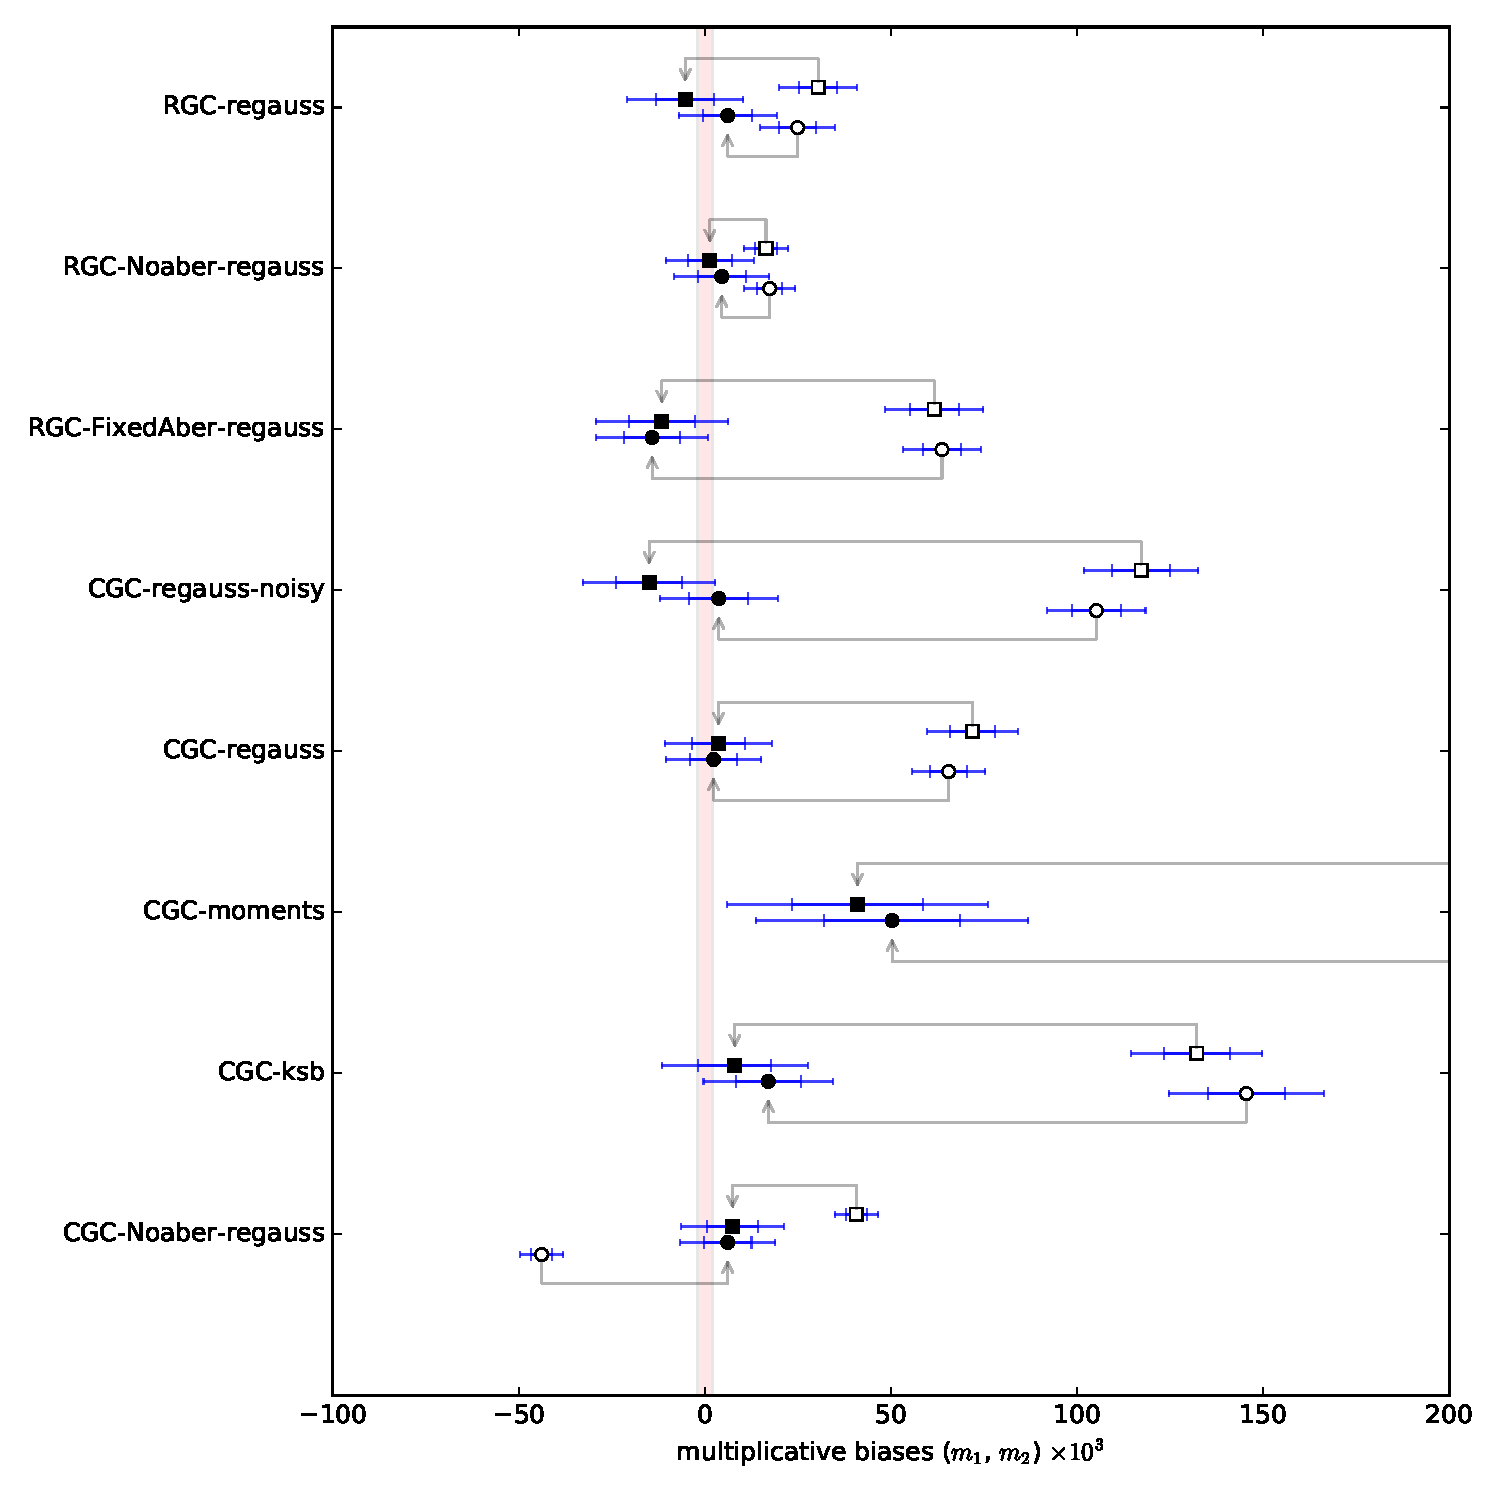
\includegraphics[width=0.8\linewidth]{./Plots/m_results_linear.pdf}
\end{center}
\caption{Calibration bias results. Each row shows muliplicative
  calibration bias $m_1$ (top) and $m_2$ (bottom) before and after
  metacalibration. Pre- and post-correction points are connected by
  gray arrows: in every case the procedure has reduced or eliminated
  the amplitude of detectable multiplicative calibration bias.}
\label{fig:m_results}
\end{figure*}

\begin{figure*}[t]
\begin{center}
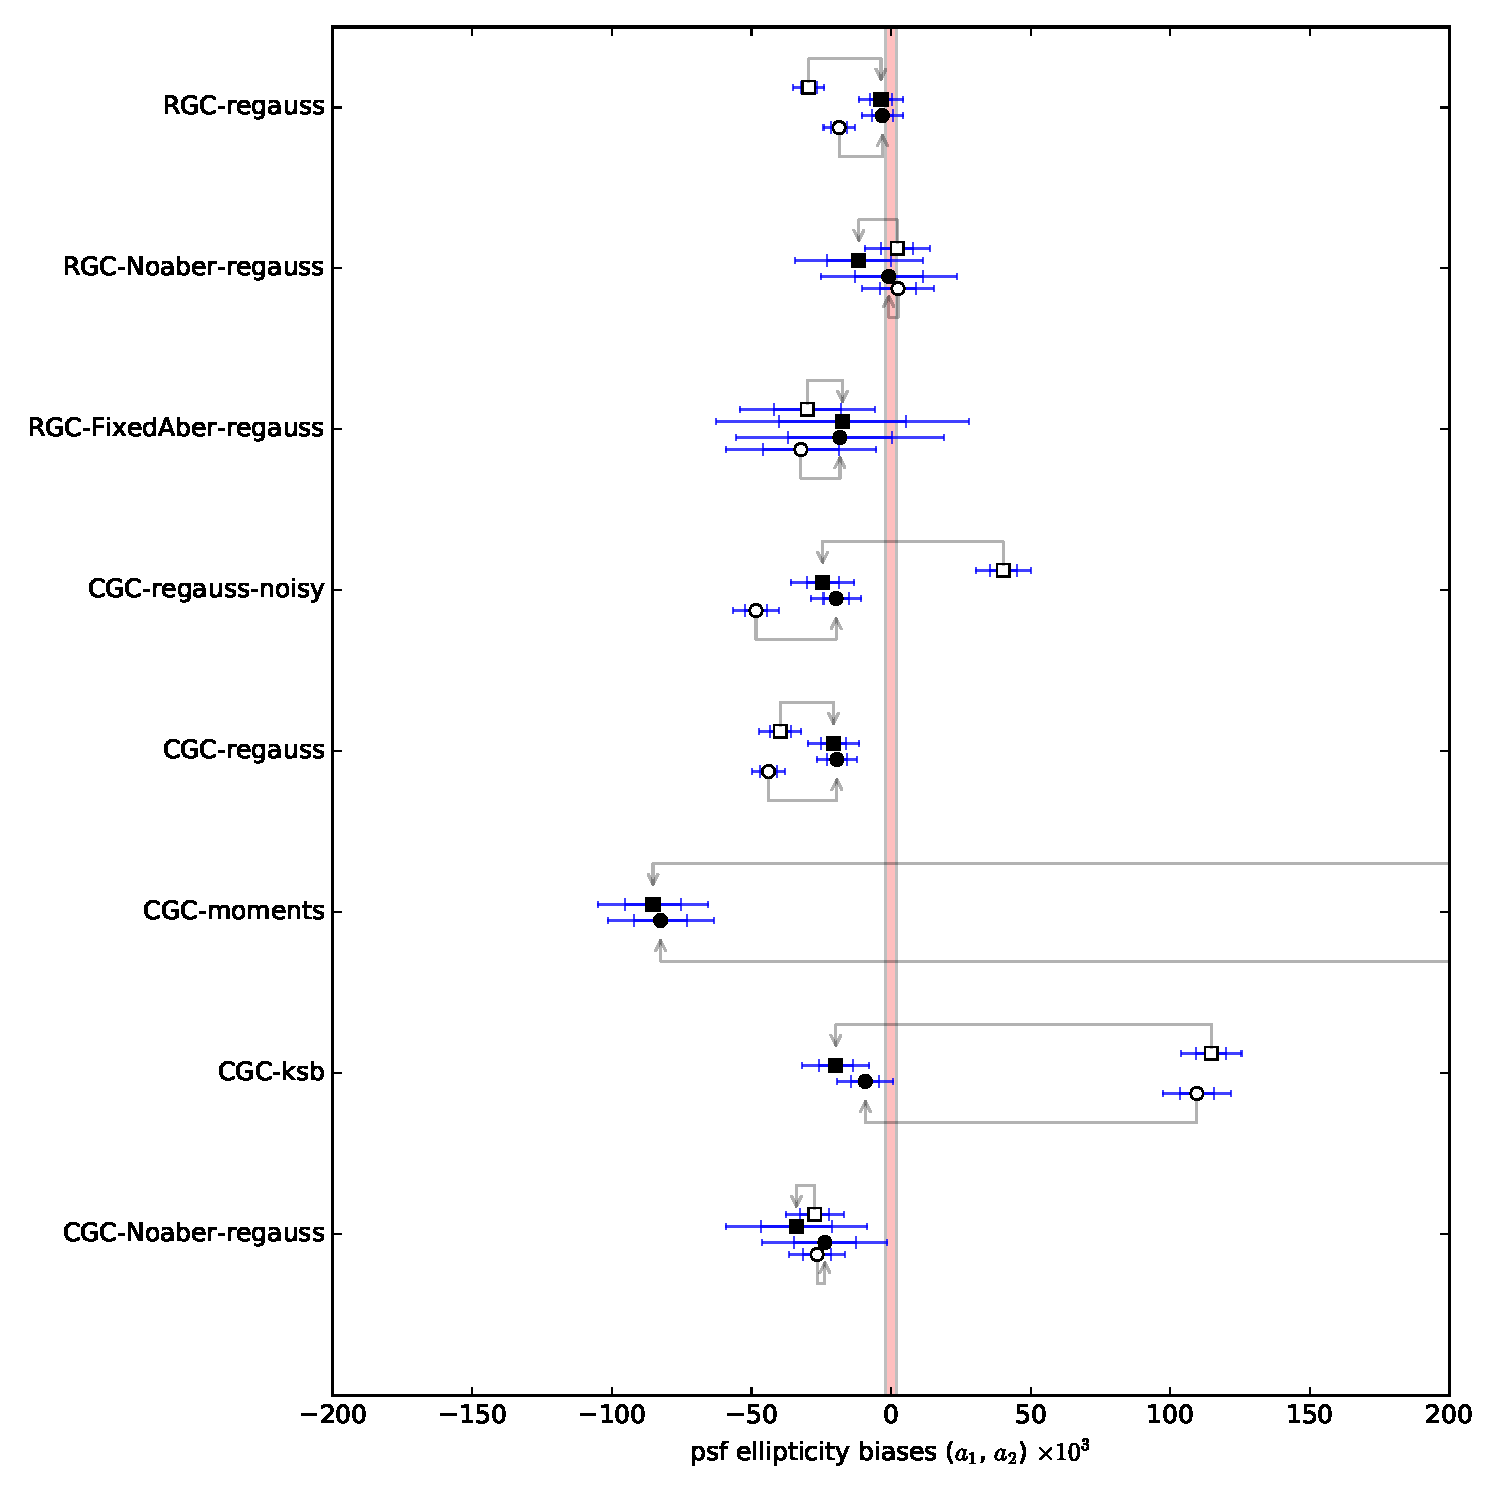
\includegraphics[width=0.8\linewidth]{./Plots/a_results_linear.pdf}
\end{center}
\caption{Calibration bias results. Each row shows linear coupling
  between the PSF ellipticity and the measured shape $a_1$ (top) and
  $a_2$ (bottom) before and after metacalibration. Pre- and
  post-correction points are connected by gray arrows: in every case
  the procedure has reduced or eliminated the amplitude of detectable
  PSF coupling.}
\label{fig:a_results}
\end{figure*}



\bibliographystyle{apj}
\bibliography{bibliography}

\end{document}.